\documentclass[10pt]{article}
\usepackage[letterpaper,margin=1in]{geometry}
\usepackage[T1]{fontenc}
\usepackage{newtxtext,newtxmath}
\usepackage{microtype}
\usepackage{graphicx}
\usepackage{booktabs}
\usepackage{multirow}
\usepackage{amsmath}
\usepackage{xcolor}
\usepackage{tikz}
\usetikzlibrary{positioning,arrows.meta,fit,backgrounds,shapes.geometric}
\usepackage[numbers,sort&compress]{natbib}
\usepackage[hidelinks]{hyperref}
\usepackage{caption}
\captionsetup{font=small,labelfont=bf}
\setlength{\tabcolsep}{4pt}
\emergencystretch=1.5em
\newcommand{\qss}{QSS}

\title{Sets, Not Neighbors: Query-Time Set Selection and\\Visibility-Gated Reading for Multimodal Agent Memory}
\author{Anonymous Authors}
\date{}

\begin{document}
\maketitle

\begin{abstract}
Recent evaluations of conversational agent memory show that retrieving raw dialogue turns by embedding similarity matches or exceeds memory systems that rewrite or compress history at ingestion. After verifying that this result holds on text benchmarks once the retrieval budget is sufficiently large, we identify why it breaks down in multimodal agent memory. Multimodal queries frequently target a relational set of past items rather than an isolated fact, and independent top-$k$ similarity ranking rarely recovers such sets intact: on MemEye, the probability that top-10 retrieval returns the complete evidence set drops from 0.92 on single-round queries to 0.32 on queries requiring four or five rounds. To address this limitation without discarding visual detail at write time, we propose a unified two-stage framework coupling Query-Time Set Selection (\qss{}) with Visibility-Gated Set Reading (VGS). \qss{} preserves raw dialogue rounds and original images for perception while constructing a compact, prefix-cacheable text index at ingestion; at query time, a selector model reads the index to resolve narrative references and return an evidence set of adaptive cardinality. On MemEye, \qss{} recovers complete evidence sets for 90.3\% of queries while opening an average of 7.3 rounds, compared to 53.9\% for cosine retrieval at equal size, and controlled comparisons with the same model show that the set formulation adds recall beyond listwise ranking and graded relevance with a dynamic cutoff. Evaluating frozen \qss{} on the held-out MemLens benchmark reveals two structural boundaries that govern index-based memory: when evidence is buried as incidental remarks inside long multi-topic turns, a terse index obscures set cues (reducing index visibility from 95\% on MemEye to 37\% on MemLens), and even when complete sets are provided, lightweight readers fail to aggregate values across multiple multimodal rounds while degrading further under naive set expansion. VGS resolves both bottlenecks by estimating index visibility from unlabeled retrieval candidates at query time: it routes high-visibility queries to standard \qss{} and adapts low-visibility queries by widening index snippets and pairing raw rounds with lightweight per-member evidence notes that make set members and numerical values explicit. Across held-out MemLens test queries, VGS improves lightweight reader accuracy by $+0.071$ $[+0.032, +0.109]$ over top-40 retrieval while preserving full performance on high-visibility benchmarks.
\end{abstract}

\section{Introduction}
\label{sec:intro}

Conversational agents that assist users over extended periods accumulate long histories of dialogue interleaved with visual artifacts such as screenshots, receipts, product photographs, and charts. To answer a user query, the memory of the agent must locate and deliver the relevant historical evidence to a reader model. In text-based conversational memory, recent controlled studies demonstrate that a remarkably simple baseline matches or surpasses complex memory architectures: storing the raw dialogue history without write-time extraction or summarization and retrieving the top-$k$ turns by embedding similarity performs on par with dedicated graph and summary memory systems~\citep{bao2026rawrag,zhou2026explicit,sharma2026selection,peng2026memorytax}. Our replication confirms that on standard text benchmarks such as LoCoMo~\citep{maharana2024locomo} and LongMemEval~\citep{wu2025longmemeval}, cosine retrieval over raw turns is statistically indistinguishable from full-context reading once the retrieval budget $k$ is large enough to cover the required evidence (Section~\ref{sec:prelim}).

Moving from text to multimodal agent memory, however, violates the core premise of independent similarity ranking. Top-$k$ retrieval assumes that the evidence for a query consists of the memory units that are individually most similar to the query in embedding space. In multimodal personal histories, user queries frequently refer not to an isolated turn, but to a relational \emph{set} of past items: all five promotional posters of a specific brand, the nutrition summary cards from day 9 and day 11, or every route checkpoint recorded during an evening run. Because the final count, comparison, or temporal trend depends on every member of the target group, missing even a single round invalidates the answer. Resolving such sets via top-$k$ embedding similarity fails for two coupled reasons. First, set members are frequently referenced through discourse or narrative aliases—such as ``the D9 summary card'' or ``the provisional busy-day trend''—that never appear in the target turn or in an image caption, and instead can only be resolved from the sequential structure of the history. Second, multimodal embeddings exhibit a pronounced modality gap~\citep{liang2022modalitygap} in which relevant images receive lower cosine similarity scores than unrelated text turns, while replacing images with write-time captions loses fine-grained visual details and increases token consumption. Consequently, as the cardinality of the required evidence set increases, the probability that top-$k$ retrieval recovers the complete set decays sharply (Figure~\ref{fig:setsize}).

Designing a multimodal memory architecture that reliably resolves and reasons over evidence sets introduces three fundamental challenges. The first challenge is joint set resolution without write-time loss: the memory must resolve discourse aliases across the global history and adapt the number of retrieved rounds to the true cardinality of the target set, while preserving original images for the reader and avoiding static write-time clustering that cannot anticipate query-defined groups. The second challenge is the index visibility boundary across heterogeneous histories: to make global navigation affordable, an index-based selector must inspect a compact representation of each round. When visual and textual evidence is foregrounded in concise turns, as in MemEye~\citep{guo2026memeye}, a short index line exposes 95\% of the query-relevant terms; when evidence is buried as an incidental remark inside long, multi-topic conversations, as in MemLens~\citep{ren2026memlens}, a terse index exposes only 37\% of those terms, causing query-time selectors to under-select. The third challenge is the reader set-aggregation bottleneck: for lightweight vision-language readers, retrieving a complete evidence set does not guarantee a correct answer. Even when given oracle evidence on MemLens, a lightweight reader answers only 6\% of arithmetic queries and 9\% of counting queries, and naively expanding the retrieved set (for instance, by including all rounds from selected sessions) reduces end-to-end accuracy because additional distractor rounds overwhelm the aggregation capacity of the reader.

\begin{figure}[t]
\centering
\resizebox{\linewidth}{!}{%
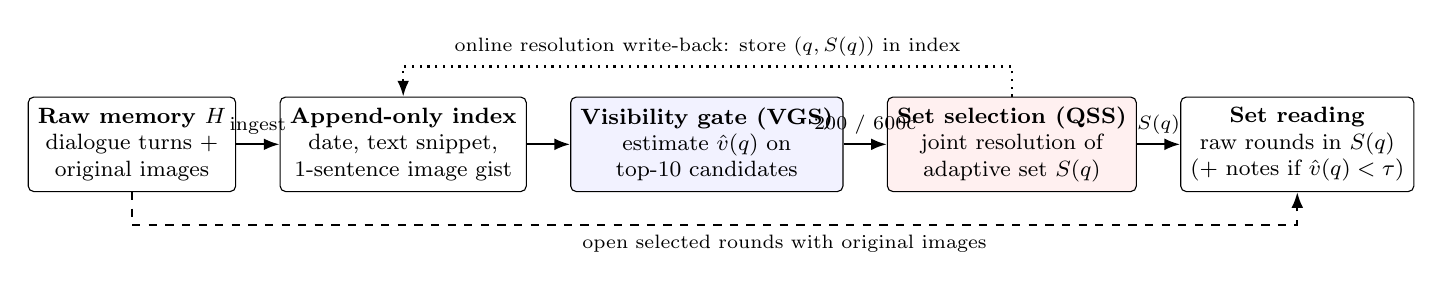
\begin{tikzpicture}[font=\footnotesize, node distance=4mm and 5.5mm,
  box/.style={draw, rounded corners=2pt, align=center, inner sep=3.5pt, fill=white, minimum height=1.2cm},
  gate/.style={draw, rounded corners=2pt, align=center, inner sep=3.5pt, fill=blue!5, minimum height=1.2cm},
  selbox/.style={draw, rounded corners=2pt, align=center, inner sep=3.5pt, fill=red!6, minimum height=1.2cm},
  arr/.style={-{Latex[length=2mm]}, thick}]
\node[box, minimum width=2.4cm] (hist) {\textbf{Raw memory $H$}\\dialogue turns +\\original images};
\node[box, right=of hist, minimum width=2.7cm] (idx) {\textbf{Append-only index}\\date, text snippet,\\1-sentence image gist};
\node[gate, right=of idx, minimum width=2.9cm] (vgs) {\textbf{Visibility gate (VGS)}\\estimate $\hat{v}(q)$ on\\top-10 candidates};
\node[selbox, right=of vgs, minimum width=2.8cm] (sel) {\textbf{Set selection (\qss{})}\\joint resolution of\\adaptive set $S(q)$};
\node[box, right=of sel, minimum width=2.7cm] (read) {\textbf{Set reading}\\raw rounds in $S(q)$\\(+ notes if $\hat{v}(q)<\tau$)};
\draw[arr] (hist) -- node[above, font=\scriptsize]{ingest} (idx);
\draw[arr] (idx) -- (vgs);
\draw[arr] (vgs) -- node[above, font=\scriptsize]{200 / 600c} (sel);
\draw[arr] (sel) -- node[above, font=\scriptsize]{$S(q)$} (read);
\draw[arr, dashed] (hist.south) -- ++(0,-0.42) -| node[pos=0.28, below, font=\scriptsize]{open selected rounds with original images} (read.south);
\draw[arr, dotted] (sel.north) -- ++(0,0.38) -| node[pos=0.25, above, font=\scriptsize]{online resolution write-back: store $(q, S(q))$ in index} (idx.north);
\end{tikzpicture}}
\caption{Overview of Query-Time Set Selection (\qss{}) and Visibility-Gated Set Reading (VGS). At ingestion, the memory keeps raw multimodal rounds intact and appends one compact line per round to a prefix-cacheable text index. At query time, VGS estimates index visibility $\hat{v}(q)$ without labels: high-visibility queries ($\hat{v}(q)\ge\tau$) use standard 200-character index lines and direct multimodal reading, whereas low-visibility queries ($\hat{v}(q)<\tau$) widen index lines to 600 characters for selection and prepend lightweight per-member evidence notes to the raw rounds for aggregation. Online resolution write-back appends resolved sets to the index to amortize future queries.}
\label{fig:overview}
\end{figure}

To address these challenges in a unified manner, we propose Query-Time Set Selection (\qss{}) coupled with Visibility-Gated Set Reading (VGS) (Figure~\ref{fig:overview}). To achieve joint set resolution without write-time loss, \qss{} decouples navigation from perception: the memory retains raw dialogue turns and original images for the reader, while writing a single compact index line per round at ingestion (date, dialogue snippet, and a one-sentence image description). Because the index is text-only and append-only, its tokens can be served from a prefix cache across queries. At query time, a language model selector inspects the index and outputs an unordered set of round identifiers $S(q)$ of model-determined size, while lightweight selectors amortize this reasoning through sampling consensus and online resolution write-back of previously resolved sets. To overcome the index visibility and reader aggregation bottlenecks, VGS estimates query-specific index visibility $\hat{v}(q)$ at runtime without ground-truth labels by computing the fraction of shared query terms visible in the index lines of the top-10 cosine candidates. When $\hat{v}(q) \ge \tau$, the standard index adequately exposes the evidence, and VGS executes standard \qss{} and direct multimodal reading. When $\hat{v}(q) < \tau$, VGS switches to a low-visibility pathway that widens the index snippets to 600 characters during selection and instructs a lightweight model to generate per-member evidence notes for each selected round before final reading. By presenting explicit per-round facts alongside the raw multimodal rounds, VGS enables lightweight readers to aggregate values across sets without losing access to the underlying images.

We evaluate \qss{} and VGS across text benchmarks (LoCoMo, LongMemEval-S) and three multimodal memory benchmarks spanning diverse visibility regimes and history scales: MemEye (371 queries and a 32-fold enlarged scale test with 1,000 distractor images), Mem-Gallery~\citep{bei2026memgallery} (903 queries), and held-out MemLens (699 queries at 32k and 200 queries at 128k). On MemEye, \qss{} recovers complete evidence sets for 90.3\% of queries in 7.3 rounds (versus 53.9\% for equal-size cosine retrieval), and same-model controls confirm that the set formulation adds $+0.059$ full-set recall over listwise ranking and $+0.097$ over a dynamic graded relevance cutoff. On held-out MemLens, where plain \qss{} under-selects due to low index visibility ($37\%$), VGS accurately routes queries by estimated visibility and improves lightweight reader accuracy on the held-out test split by $+0.071$ $[+0.032, +0.109]$ over top-40 retrieval, driven by large gains on arithmetic ($0.03 \to 0.21$), counting ($0.10 \to 0.23$), and ordering ($0.12 \to 0.38$) queries. Extensive ablations further establish the boundaries of the framework: write-time grouping, predicted aliases, structural prompting, session closure, and agentic image zooming fail to match query-time set resolution, whereas strong readers on low-visibility histories still favor broad top-$40$ retrieval because they can directly exploit unindexed contextual turns.

The contributions of this work are fourfold. First, we verify the large-budget sufficiency of raw similarity retrieval in text memory and establish that its primary failure mode in multimodal memory is set completeness, formalized via full-set recall and index visibility. Second, we introduce Query-Time Set Selection (\qss{}) and isolate, through strict same-model ranking and dynamic-cutoff controls across two benchmarks, the specific recall advantage of formulating retrieval as variable-size set resolution alongside lightweight consensus and resolution write-back mechanisms. Third, we propose Visibility-Gated Set Reading (VGS), which acts on a label-free query-time estimate of index visibility to adapt index horizon and per-member note generation, yielding statistically significant end-to-end gains for lightweight readers on held-out low-visibility data while preserving high-visibility performance. Finally, we provide a rigorous empirical characterization of design boundaries across model families, reader capacities, write-time organizations, and visual resolution controls.

\section{Motivating Analysis: When Does Raw Similarity Retrieval Suffice?}
\label{sec:prelim}

To determine precisely where raw similarity retrieval ceases to be sufficient for agent memory, we conduct a controlled preliminary study comparing cosine retrieval of raw memory units against full-context reading under a fixed reader, prompt, and evaluation judge. Throughout this analysis, we use \texttt{gemini-3.8-flash} as the reader and \texttt{gemini-embedding-2} as the embedding model; Section~\ref{sec:setup} details the shared evaluation protocol, and all reported differences $\Delta$ are paired across questions with 95\% bootstrap confidence intervals.

\begin{table}[t]
\centering
\caption{Comparison of raw cosine retrieval and full-context reading under a fixed reader (\texttt{gemini-3.8-flash}). $\Delta$ denotes the paired accuracy difference relative to full-context reading with 95\% bootstrap confidence intervals; Tokens indicates mean prompt tokens per question. LoCoMo and LongMemEval-S use the strict LongMemEval judge; MemEye uses its official 0--1 rubric. ``Annotated evidence'' provides only the ground-truth evidence turns or rounds.}
\label{tab:prelim}
\small
\resizebox{\linewidth}{!}{%
\begin{tabular}{llccr}
\toprule
Benchmark & Condition & Accuracy & $\Delta$ vs.\ full context & Tokens \\
\midrule
\multirow{4}{*}{LoCoMo (1,540 q)} & Full context & 0.790 & -- & 32,499 \\
 & Cosine top-100 turns & 0.781 & $-0.009$ $[-0.023, +0.006]$ & 5,693 \\
 & Cosine top-10 turns & 0.706 & $-0.084$ $[-0.105, -0.064]$ & 755 \\
 & Annotated evidence & 0.739 & $-0.051$ $[-0.071, -0.031]$ & 435 \\
\midrule
\multirow{3}{*}{LongMemEval-S (119 q)} & Full context & 0.950 & -- & 113,227 \\
 & Cosine top-50 rounds & 0.941 & $-0.008$ $[-0.034, +0.017]$ & 21,730 \\
 & Cosine top-10 rounds & 0.899 & $-0.050$ $[-0.092, -0.017]$ & 4,986 \\
\midrule
\multirow{7}{*}{MemEye (371 q)} & Full context, images at low resolution & 0.819 & -- & 27,232 \\
 & Full context, images at high resolution & 0.811 & $-0.008$ $[-0.036, +0.020]$ & 78,961 \\
 & Full context, dense captions instead of images & 0.779 & $-0.040$ $[-0.077, -0.005]$ & 55,309 \\
 & Full context, no visual information & 0.191 & -- & 11,262 \\
 & Cosine top-40 rounds, images & 0.741 & $-0.079$ $[-0.112, -0.047]$ & 11,136 \\
 & Cosine top-10 rounds, images & 0.689 & $-0.130$ $[-0.173, -0.090]$ & 3,916 \\
 & Annotated evidence, images & 0.746 & $-0.073$ $[-0.115, -0.034]$ & 2,039 \\
\bottomrule
\end{tabular}}
\end{table}

\paragraph{Sufficiency of large-budget retrieval in text memory.} Table~\ref{tab:prelim} summarizes performance on two standard text memory benchmarks: LoCoMo~\citep{maharana2024locomo} (1,540 questions) and a stratified subset of LongMemEval-S~\citep{wu2025longmemeval} (119 questions). When the retrieval budget is generous—top-100 turns on LoCoMo and top-50 rounds on LongMemEval-S—raw cosine retrieval comes within 0.009 and 0.008 of full-context reading, with both 95\% confidence intervals spanning zero while reducing prompt tokens by 5.2- to 5.7-fold. Substantial degradation emerges only under tight retrieval budgets, such as top-10 retrieval ($\Delta = -0.084$ on LoCoMo and $-0.050$ on LongMemEval-S). Notably, feeding the reader only the human-annotated evidence turns on LoCoMo yields 0.739 accuracy, which is 0.051 below full-context reading ($[-0.071, -0.031]$) and 0.042 below top-100 retrieval. This pattern indicates that raw similarity retrieval succeeds in text memory because individual turns are inexpensive in tokens, allowing a large $k$ to capture both the core evidence and surrounding conversational context without write-time compression.

\paragraph{Navigation--perception asymmetry in multimodal memory.} The bottom block of Table~\ref{tab:prelim} evaluates the same reader on MemEye~\citep{guo2026memeye} (371 questions across eight life scenarios), where removing all visual inputs collapses accuracy to 0.191. Comparing representation and retrieval strategies reveals three empirical regularities that distinguish multimodal memory from text memory. First, reading the full history with original images at low resolution ($\sim 266$ tokens per image) achieves 0.819 accuracy, exceeding top-40 retrieval by $+0.079$ $[+0.047, +0.112]$ and top-10 retrieval by $+0.130$ $[+0.090, +0.173]$, whereas increasing image resolution to high ($\sim 1,070$ tokens per image) triples the token cost without improving accuracy ($0.811$). Second, replacing original images at ingestion with dense textual captions ($\sim 800$ tokens per image) reduces full-context accuracy to 0.779 ($\Delta = -0.040$ $[-0.077, -0.005]$) while doubling prompt tokens ($55,309$ versus $27,232$). Third, although captions degrade perception when they replace images, they are essential as retrieval keys: as shown in Appendix Table~\ref{tab:keys}, indexing rounds by dialogue text plus a caption achieves 0.774 gold coverage@10, compared to 0.671 for an interleaved text-and-image embedding and 0.300 for an image-only embedding. In the shared embedding space of \texttt{gemini-embedding-2}, relevant image rounds receive a lower mean cosine similarity (0.548--0.568) than unrelated pure-text rounds (0.575), reflecting the cross-modal embedding gap~\citep{liang2022modalitygap}. Furthermore, the benefit of full-context reading depends on reader capacity: when replacing the strong reader with lightweight models (\texttt{gemini-3.1-flash-lite} or \texttt{gemini-2.5-flash-lite}), reading only the focused annotated evidence surpasses full-context reading by $+0.055$ and $+0.044$ (Appendix Table~\ref{tab:reader}).

\paragraph{The set-completeness bottleneck.} To identify why even top-40 retrieval with caption keys trails full-context reading by 0.079 on MemEye, we stratify the accuracy gap between full-context reading and top-10 retrieval by the cardinality of the ground-truth evidence set $|G(q)|$. The accuracy deficit is minor for single-round queries ($0.038$, $n{=}119$), widens to $0.125$ for queries requiring two or three rounds ($n{=}166$), and reaches $0.267$ for queries requiring four or more rounds ($n{=}86$). Equivalently, the deficit is only $0.034$ when the retrieved pool contains the entire gold evidence set ($n{=}235$), but jumps to $0.296$ whenever at least one gold round is missing ($n{=}136$). Figure~\ref{fig:setsize} illustrates why simply enlarging $k$ does not resolve this issue: under top-10 cosine retrieval, the fraction of questions for which the complete evidence set is recovered falls from $0.916$ ($|G|{=}1$) to $0.614$ ($2\text{--}3$), $0.316$ ($4\text{--}5$), and $0.000$ ($\ge 6$), and even top-40 retrieval recovers only $0.300$ of sets with six or more rounds. Qualitative inspection of the missed rounds reveals that set queries routinely identify target items via narrative aliases defined elsewhere in the timeline: for example, ``the D9 summary card'' refers to a card shared during the ninth session, and ``the provisional busy-day trend'' refers to a chart from a session that opened with the remark ``Busy day. I thought this snack might fit, but I am not fully sure.'' Because neither phrase occurs in the target round or its visual caption, independent per-round similarity scoring cannot link the alias to its referent.

\begin{figure}[t]
\centering
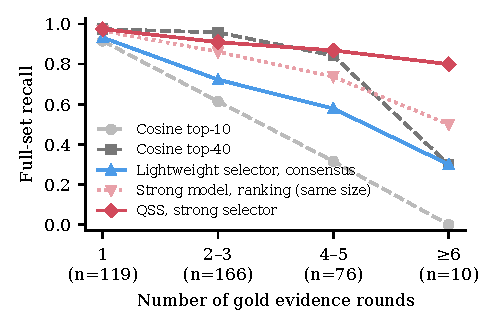
\includegraphics[width=0.48\linewidth]{figures/setsize.pdf}
\caption{Full-set recall on MemEye stratified by the number of ground-truth evidence rounds $|G(q)|$ (371 questions; subgroup sizes in parentheses). Dashed lines denote cosine top-10 and top-40 retrieval. \qss{} applies \texttt{gemini-3.8-flash} to a cosine prefilter of 100 candidates and opens 7.7 rounds on average; the ranking control instructs the same model to rank the same candidates and truncates each query at the exact cardinality chosen by \qss{}. The lightweight selector applies sampling consensus with \texttt{gemini-2.5-flash-lite} (Section~\ref{sec:method}).}
\label{fig:setsize}
\end{figure}

\paragraph{Design requirements.} Together, these findings establish four concrete requirements for multimodal agent memory. First, retrieval evaluation and optimization must target full-set recall rather than average item recall. Second, the retriever must resolve discourse aliases against the sequential structure of the history and adapt the number of opened rounds to the cardinality of the target set. Third, write-time descriptions should serve solely as navigation keys while the reader perceives the original images. Fourth, the reading interface must account for both the visibility of evidence in the navigation index and the limited multi-round aggregation capacity of lightweight readers.

\section{Methodology: Query-Time Set Selection and Visibility-Gated Reading}
\label{sec:method}

To satisfy the four design requirements derived in Section~\ref{sec:prelim}, we design a two-stage multimodal memory framework comprising Query-Time Set Selection (\qss{}) for adaptive set retrieval and Visibility-Gated Set Reading (VGS) for visibility-aware evidence extraction and reading. We first formalize the set retrieval task, then detail the memory index, the query-time selection mechanism, the visibility-gated reading pipeline, and the lightweight amortization strategies.

\subsection{Problem Formulation and Full-Set Recall}
\label{sec:formulation}

We represent the interaction history of a user as an ordered sequence of multimodal dialogue rounds $H = (r_1, \dots, r_n)$. Each round $r_i = (u_i, a_i, \mathcal{I}_i, t_i, s_i)$ consists of a user message $u_i$, an assistant response $a_i$, a (possibly empty) set of shared images $\mathcal{I}_i$, a timestamp $t_i$, and a session identifier $s_i$. Given a user query $q$ (which may itself include an image), a memory selector returns a candidate subset of rounds $S(q) \subseteq H$, and a reader model generates the final answer conditioned on $q$ and the raw multimodal content of $S(q)$.

Let $G(q) \subseteq H$ denote the ground-truth set of rounds containing the decisive evidence required to answer $q$. Standard retrieval metrics such as coverage, defined as $\mathrm{Cov}(q) = |G(q) \cap S(q)| / |G(q)|$, average over individual items and obscure whether a multi-round set was retrieved intact. Because missing a single member corrupts counting, arithmetic, and comparison queries, we formulate our primary retrieval objective around Full-Set Recall (FSR):
\begin{equation}
\mathrm{FSR}(q) = \mathbb{1}\left[G(q) \subseteq S(q)\right],
\label{eq:fsr}
\end{equation}
where $\mathbb{1}[\cdot]$ is the indicator function that equals $1$ if and only if every ground-truth round in $G(q)$ is included in $S(q)$. Averaged across a benchmark, $\mathrm{FSR}$ corresponds to the per-query form of all-recall in multi-hop retrieval~\citep{gutierrez2024hipporag} and supporting-fact exact match in multi-hop question answering~\citep{yang2018hotpotqa}. Because reader inference cost and distractor interference scale with the number of opened rounds $|S(q)|$, the goal of the memory system is to maximize $\mathrm{FSR}(q)$ and end-to-end answer accuracy while keeping $|S(q)|$ compact. Under standard top-$k$ cosine retrieval, $|S(q)| = k$ is fixed across all queries and rounds are scored independently by $\cos(e(q), e(r_i))$, so $\mathrm{FSR}(q) = 1$ requires the worst-ranked member of $G(q)$ to rank within the top $k$. On MemEye, the rank of this worst-ranked member has a median of 5 and exceeds 40 on 7.8\% of queries.

\subsection{Append-Only Multimodal Memory Index}
\label{sec:index}

To enable global reasoning over the history at query time without loading raw images into the selector, the memory constructs a lightweight text index $I(H) = (\ell_1, \dots, \ell_n)$ at ingestion, with one index line $\ell_i$ per round $r_i$. In the default configuration, $\ell_i$ concatenates the round identifier and timestamp $t_i$, the first $L_{\mathrm{usr}}{=}200$ characters of the user message $u_i$, a one-sentence visual gist of each image in $\mathcal{I}_i$ generated once at write time from the image alone, and the first $L_{\mathrm{ast}}{=}100$ characters of the assistant response $a_i$.

This index design enforces a strict separation between navigation and perception. First, the visual gist is used exclusively for indexing and is never substituted for the original images $\mathcal{I}_i$ during reading. Second, each index line consumes approximately 70 tokens on MemEye, allowing a 300-round history to fit within 22k tokens and a 1M-token context window to accommodate roughly 14,000 rounds. Third, because $\ell_i$ depends only on $r_i$, the index $I(H)$ grows strictly by appending as new rounds arrive, allowing the entire historical index prefix to be served from a key-value prefix cache across consecutive user queries.

\subsection{Query-Time Set Selection and Same-Model Controls}
\label{sec:qss}

At query time, \qss{} presents the index $I(H)$ and the query $q$ to a selector language model, which outputs a JSON list of round identifiers defining $S(q)$. Rather than scoring rounds in isolation, the selector prompt instructs the model to resolve the complete evidence set jointly: specifically, to include all members of any category or sequence referenced by $q$ (such as all advertisements of a brand or all iterations of a screen), the rounds that establish narrative labels used in $q$ (such as episode numbers or temporal markers like ``first'' and ``updated''), and candidate rounds whose brief image gist cannot rule out relevance (Appendix~\ref{app:prompts}). The selector may return up to $N{=}40$ rounds but chooses the cardinality $|S(q)|$ dynamically per query. When the history length $n$ is very large, \qss{} first applies a cosine similarity prefilter over the caption-augmented round embeddings to retain the top-$P$ candidates ($P{=}100$ for standard histories and $P{=}200$ for enlarged histories), and presents their index lines in chronological order to the selector. This prefilter bounds the complexity of the selection call by $O(P)$ tokens while preserving chronological context for joint set resolution.

To isolate the specific contribution of formulating retrieval as variable-size set selection—as opposed to simply using a capable language model as a reranker~\citep{sun2023rankgpt,zhuang2024beyond}—we design two strict controls that use the exact same model, candidate pool, and index lines:
\begin{equation}
S_{\mathrm{rank}}(q) = \mathrm{Top}_{|S_{\mathrm{QSS}}(q)|}\big(\pi_{\mathrm{LLM}}(I(H), q)\big), \qquad
S_{\mathrm{grade}}(q) = \big\{\, r_i \in H \;\big|\; g_{\mathrm{LLM}}(\ell_i \mid I(H), q) \ge 2 \,\big\}.
\label{eq:controls}
\end{equation}
In Equation~\eqref{eq:controls}, $\pi_{\mathrm{LLM}}$ denotes a listwise ranking of all candidates from most to least useful produced by the selector model, which is then truncated for each question at the exact cardinality $|S_{\mathrm{QSS}}(q)|$ chosen by \qss{} (granting the ranking control oracle knowledge of the selected set size). Conversely, $g_{\mathrm{LLM}} \in \{0, 1, 2, 3\}$ denotes a listwise graded relevance score assigned to each candidate in a single call ($0$: irrelevant, $3$: decisive evidence), from which $S_{\mathrm{grade}}(q)$ retains all rounds scored $2$ or higher as a dynamic cutoff.

\subsection{Index Visibility and Visibility-Gated Set Reading}
\label{sec:vgs}

While \qss{} resolves sets effectively when index lines expose the relevant cues, a compact snippet of $L_{\mathrm{usr}}{=}200$ characters can truncate evidence that occurs mid-way through a long multi-topic turn. Furthermore, even when $S(q)$ is complete, lightweight readers frequently fail to aggregate numerical or categorical facts scattered across multiple multimodal rounds, and naively enlarging $S(q)$ degrades their accuracy further due to distractor interference.

To formalize when a compact index suffices, we define the ground-truth index visibility $v(q)$ of a query as the average fraction of query content words present in a gold round that are also preserved within its index line:
\begin{equation}
v(q) = \frac{1}{|G(q)|} \sum_{r_i \in G(q)} \frac{|W(q, r_i) \cap W(\ell_i)|}{|W(q, r_i)|},
\label{eq:vis}
\end{equation}
where $W(q, r_i)$ is the set of content words shared between query $q$ and the full text (plus caption) of round $r_i$, and $W(\ell_i)$ is the set of content words appearing in the index line $\ell_i$. Because $G(q)$ is unknown at inference time, Visibility-Gated Set Reading (VGS) computes a label-free query-time estimate $\hat{v}(q)$ by replacing $G(q)$ in Equation~\eqref{eq:vis} with $C_{10}(q)$, the set of top-10 rounds ranked by cosine similarity that share at least one content word with $q$:
\begin{equation}
\hat{v}(q) = \frac{1}{|C_{10}(q)|} \sum_{r_i \in C_{10}(q)} \frac{|W(q, r_i) \cap W(\ell_i)|}{|W(q, r_i)|}.
\label{eq:vhat}
\end{equation}
Computing $\hat{v}(q)$ requires zero model calls and executes in milliseconds using the existing cosine retrieval rankings. VGS compares $\hat{v}(q)$ against a fixed threshold $\tau{=}0.7$ calibrated on development data (which cleanly separates concise-turn histories, where 98.7\% of MemEye queries satisfy $\hat{v}(q) \ge 0.7$, from long-turn histories, where 87.6\% of MemLens development queries satisfy $\hat{v}(q) < 0.7$) to route each query between two reading pathways. In the high-visibility pathway ($\hat{v}(q) \ge \tau$), because the compact index already exposes the query cues, VGS executes standard \qss{} ($L_{\mathrm{usr}}{=}200$) and passes the selected raw multimodal rounds $S(q)$ in chronological order directly to the reader; for strong readers that benefit from global narrative framing (such as session sequence and surrounding dates), an index-as-context option prepends $I(H)$ to $S(q)$. In the low-visibility pathway ($\hat{v}(q) < \tau$), to expose evidence buried inside long turns, VGS widens the user snippet horizon in the index to $L_{\mathrm{usr}}{=}600$ characters during \qss{} selection. Then, to overcome the set-aggregation bottleneck of lightweight readers without discarding raw visual detail, VGS invokes the lightweight model to inspect each selected round $r_i \in S(q)$ (including its original images $\mathcal{I}_i$) and write a concise per-member evidence note $m_i(q)$ recording the specific entities, dates, or numerical values relevant to $q$. The reader receives the compiled notes $\{m_i(q)\}_{r_i \in S(q)}$ followed by the raw multimodal rounds $S(q)$, allowing it to perform arithmetic, counting, or ordering over explicit facts while verifying fine visual details from the raw images.

\subsection{Amortizing Selection for Lightweight Models}
\label{sec:lightweight}

When deployment constraints require running the selection step itself on a lightweight model rather than a frontier model, single-pass selection suffers from degraded recall and noisy membership decisions. We introduce two complementary mechanisms that keep all query-time calls on the lightweight model:

\paragraph{Sampling consensus.} Following self-consistency principles~\citep{wang2023selfconsistency} adapted to set prediction, the lightweight selector draws $K{=}5$ independent set samples $\{S^{(1)}(q), \dots, S^{(K)}(q)\}$ at temperature $T{=}1.0$ and retains rounds receiving at least $V$ votes: $S_{\mathrm{cons}}(q) = \{r_i \in H \mid \sum_{k=1}^K \mathbb{1}[r_i \in S^{(k)}(q)] \ge V\}$. Setting $V{=}2$ filters out idiosyncratic false positives that arise in the full union ($V{=}1$) while recovering set members missed by greedy decoding.

\paragraph{Online resolution write-back.} Although static write-time clustering fails to anticipate arbitrary user queries, a personal memory system answers multiple queries over the lifetime of a user history. Once a query $q'$ has been answered using selected set $S(q')$, resolution write-back appends the resolved pair $(q', S(q'))$ as a compact entry at the end of the memory index $I(H)$. Subsequent queries $q$ observe the accumulated resolutions of earlier queries, enabling the selector to reuse previously resolved narrative aliases (such as which rounds constitute ``Episode 2'' or ``the D9 summary''). In our online evaluation protocol, queries arrive in random order, each query observes only preceding resolutions, and any prior query with embedding cosine similarity above $0.9$ to $q$ is masked out to prevent paraphrase leakage. We also evaluate a model-free variant that directly takes the union of the resolved sets of the three nearest prior queries and the cosine top-5 rounds.

\subsection{Cost and Prefix-Caching Model}
\label{sec:costmodel}

The inference cost of the framework decomposes into index selection, optional note extraction (when $\hat{v}(q) < \tau$), and multimodal reading. Because the selection call processes only text tokens ($I(H)$ and $q$) and outputs a short list of identifiers, its uncached cost on MemEye is \$9.47 per 1,000 queries with the strong selector (\texttt{gemini-3.8-flash}, averaging 11.5k input and 230 output tokens), which drops to \$1.82 per 1,000 queries when the append-only index is served from the prefix cache. At the reading stage, the reader processes only $|S(q)|$ multimodal rounds (7.3 on average for \qss{} on MemEye) rather than $k{=}40$ rounds under wide similarity retrieval. In the low-visibility pathway of VGS, per-member note generation uses the lightweight model (\texttt{gemini-2.5-flash-lite}, \$0.10 per million input tokens), adding only \$0.47 per 1,000 queries on MemLens. We report measured API expenditure across all experiments alongside warm-cache estimates for persistent per-user deployments (Appendix~\ref{app:cost}).

\section{Experimental Setup}
\label{sec:setup}

We structure our empirical evaluation around six research questions designed to test each component and boundary condition of our framework. RQ1 asks whether \qss{} recovers complete evidence sets with compact, adaptive budgets across benchmarks, and how much recall the set formulation adds beyond same-model listwise ranking and dynamic graded cutoffs. RQ2 asks how improved set recall translates into end-to-end answer accuracy, scale robustness, and inference cost across lightweight and strong readers on high-visibility histories. RQ3 examines how frozen \qss{} performs on held-out multi-session histories where evidence is buried inside long turns (MemLens), and how index visibility explains the resulting performance regime. RQ4 tests whether VGS overcomes low index visibility and the reader set-aggregation bottleneck on held-out MemLens test data while preserving performance on high-visibility benchmarks. RQ5 investigates whether query-time set selection can be replaced by write-time organization, structural prompting, or uncalibrated cross-family models, and how much of the gap sampling consensus and resolution write-back close. Finally, RQ6 examines whether agentic image zooming or write-time dense captions improve over reading original images at standard resolution.

\paragraph{Benchmarks and evaluation splits.} We evaluate across five benchmarks (two text benchmarks in Section~\ref{sec:prelim} and three multimodal benchmarks in Section~\ref{sec:results}). First, MemEye~\citep{guo2026memeye} contains 371 open-ended questions across eight multi-session life scenarios (30--299 rounds and 30--89 images per scenario, mean 126.5 rounds), where visual necessity was verified by the benchmark authors and every question has human-annotated gold evidence rounds. To test robustness to history scale (MemEye+1k), we interleave sessions from Mem-Gallery containing 1,000 distractor images into each MemEye history, expanding the mean length 32-fold from 126.5 to 4,088.5 rounds ($\sim 722\text{k}$ tokens). Second, Mem-Gallery~\citep{bei2026memgallery} provides an external multi-session benchmark across 20 scenarios, from which we evaluate a stratified sample of 903 questions. Third, MemLens~\citep{ren2026memlens} serves as our held-out benchmark of long multi-session conversations in which each question has an independent conversation haystack and removing evidence images reduces frontier model accuracy below 2\%. For RQ1 and RQ3, we evaluate frozen \qss{} across all 699 non-abstention questions at the 32k context length (64.6 rounds and 13.3 images per haystack; mean 5.9 gold rounds) and on a fixed random subset of 200 questions at the 128k context length (245.0 rounds and 48.8 images per haystack). For the VGS mechanism evaluation in RQ4, we partition the 699 MemLens questions via stratified sampling by question type and subtype into a development third (233 questions, used alongside MemEye to select the VGS design and threshold $\tau{=}0.7$) and a held-out test split (466 questions, evaluated once after freezing VGS).

\paragraph{Models and baselines.} We evaluate two primary readers: a lightweight reader (\texttt{gemini-2.5-flash-lite} at temperature 0 with default medium image resolution, evaluated both without thinking—where decoding is strictly deterministic—and with a 1,024-token thinking budget) and a strong reader (\texttt{gemini-3.8-flash} at temperature 0 with low thinking and low-resolution images). The primary \qss{} selector is \texttt{gemini-3.8-flash} with low thinking; lightweight selectors use \texttt{gemini-2.5-flash-lite} without thinking. To assess zero-shot cross-family transfer under an identical selector prompt, we additionally evaluate \texttt{gpt-5}, \texttt{gpt-5-mini}, and Qwen3-235B-A22B (instruction and thinking variants). Write-time visual gists are generated once per image by \texttt{gemini-3.8-flash} from the image alone, and dense retrieval baselines use \texttt{gemini-embedding-2} over round dialogue text concatenated with the image caption. We compare \qss{} and VGS against full-context reading (FC, feeding all rounds and images), cosine similarity retrieval (RAG@$k$ for $k \in \{10, 20, 40\}$), the two same-model controls ($S_{\mathrm{rank}}$ and $S_{\mathrm{grade}}$ defined in Section~\ref{sec:qss}), set union baselines ($\text{\qss{}} \cup \text{RAG@}k$), and oracle annotated evidence ($G(q)$). All methods evaluated with the same reader share an identical answering prompt.

\paragraph{Evaluation metrics, judges, and statistical testing.} Retrieval performance is quantified by Full-Set Recall ($\mathrm{FSR}$, Equation~\eqref{eq:fsr}), item coverage $\mathrm{Cov}(q)$, and mean opened rounds $|S(q)|$. End-to-end answer quality on MemEye and Mem-Gallery is scored using the official MemEye $\{0, 0.25, 0.5, 0.75, 1\}$ rubric with \texttt{gemini-3.8-flash} as primary judge, verified by an independent cross-family judge (Qwen3-VL-235B-A22B). On MemLens, we follow the official benchmark protocol using type-specific binary judge prompts with Qwen3-VL-235B-A22B as primary judge, verified against \texttt{gemini-3.8-flash} (which exhibits 96--97\% agreement). Cost is reported in USD per 1,000 queries at official API list prices over all retrieval, note-generation, and reading calls (excluding evaluation judging). For all paired comparisons, we compute 95\% confidence intervals via 10,000 question-level bootstrap resamples; because MemEye queries share eight underlying scenario histories, we additionally perform a two-stage cluster bootstrap (resampling scenarios first, then questions within scenarios) and Wilcoxon signed-rank tests across scenario means (Appendix Table~\ref{tab:cluster}).

\section{Experimental Results}
\label{sec:results}

\subsection{RQ1: Set-Level Retrieval and Formulation Controls}
\label{sec:rq1}

To evaluate whether query-time set selection resolves the set-completeness bottleneck identified in Section~\ref{sec:prelim}, we first assess retrieval quality independently of reader answering on both MemEye and MemLens-32k. Table~\ref{tab:select} reports the mean number of opened rounds $|S(q)|$, overall Full-Set Recall (with the FSR of cosine retrieval truncated at the exact same per-question cardinality $|S(q)|$ shown in brackets), FSR on the subset of queries requiring $|G(q)| \ge 4$ rounds, item-level coverage, and measured selection cost per 1,000 queries. The ranking control ($S_{\mathrm{rank}}$) and dynamic graded cutoff control ($S_{\mathrm{grade}}$) isolate the effect of the set formulation from the underlying relevance judgment of the language model, while Figure~\ref{fig:setsize} illustrates FSR across set sizes on MemEye.

\begin{table}[t]
\centering
\caption{Set-level retrieval performance without reader answering. FSR denotes Full-Set Recall; values in brackets report the FSR of cosine retrieval opening the exact same number of rounds per question. The ranking and dynamic cutoff controls use \texttt{gemini-3.8-flash} on the identical candidate pool as \qss{} (MemEye: cosine top-100 prefilter; MemLens: all rounds). Lightweight selectors use \texttt{gemini-2.5-flash-lite}. All costs are measured API expenditures.}
\label{tab:select}
\small
\resizebox{\linewidth}{!}{%
\begin{tabular}{lrcccr}
\toprule
Selector & Rounds & FSR [cosine] & FSR, $\ge$4 gold rounds [cosine] & Coverage & \$ / 1k q \\
\midrule
\multicolumn{6}{l}{\textit{MemEye (371 questions, 86 with $\ge$4 gold rounds)}} \\
Cosine top-10 / top-40 & 10 / 40 & 0.633 / 0.922 & 0.279 / 0.779 & 0.774 / 0.959 & 0 \\
\qss{}, full index & 7.3 & \textbf{0.903} [0.539] & \textbf{0.872} [0.151] & 0.943 & 6.43 \\
\qss{}, cosine prefilter $P{=}100$ & 7.7 & 0.919 [0.569] & 0.860 [0.209] & 0.954 & 6.37 \\
\quad Ranking control ($S_{\mathrm{rank}}$), cut at \qss{} size & 7.7 & 0.860 [0.569] & 0.709 [0.209] & -- & 9.51 \\
\quad Dynamic cutoff control ($S_{\mathrm{grade}}$), grade $\ge$2 & 4.8 & 0.806 [0.445] & 0.686 [0.070] & 0.881 & 10.41 \\
Lightweight selector / with sampling consensus & 9.8 / 10.7 & 0.712 / 0.749 & 0.512 / 0.547 & 0.818 / 0.855 & 0.37 / 1.41 \\
Lightweight selector with resolution write-back & 9.5 & 0.752 [0.606] & 0.558 [0.209] & 0.864 & 0.48 \\
\texttt{gpt-5-mini}, same prompt & 5.9 & 0.728 [0.531] & 0.605 [0.209] & 0.764 & 2.94 \\
\midrule
\multicolumn{6}{l}{\textit{MemLens-32k (held out; 699 questions, 374 with $\ge$4 gold rounds)}} \\
Cosine top-10 / top-40 & 10 / 40 & 0.342 / 0.645 & 0.000 / 0.356 & 0.590 / 0.917 & 0 \\
\qss{}, frozen 200-character index & 6.1 & 0.375 [0.176] & 0.043 [0.000] & 0.706 & 6.43 \\
\qss{}, 600-character index & 3.9 & 0.286 [0.127] & 0.037 [0.000] & 0.636 & 8.07 \\
\quad Ranking control ($S_{\mathrm{rank}}$), cut at \qss{} size & 6.1 & 0.355 [0.176] & 0.016 [0.000] & -- & 9.95 \\
\quad Dynamic cutoff control ($S_{\mathrm{grade}}$), grade $\ge$2 & 3.4 & 0.268 [0.130] & 0.008 [0.000] & 0.539 & 10.64 \\
Lightweight selector / with sampling consensus & 5.8 / 6.4 & 0.329 / 0.346 & 0.040 / 0.059 & 0.583 / 0.608 & 0.76 / 0.84 \\
Qwen3-235B-A22B, same prompt & 1.4 & 0.149 [0.107] & 0.000 [0.000] & 0.286 & 0.82 \\
\texttt{gpt-5-mini}, same prompt & 7.4 & 0.442 [0.205] & 0.126 [0.016] & 0.684 & 3.63 \\
\bottomrule
\end{tabular}}
\end{table}

Table~\ref{tab:select} and Figure~\ref{fig:setsize} yield three findings. First, on MemEye, \qss{} achieves a full-set recall of 0.903 over the full index (and 0.919 with a $P{=}100$ cosine prefilter) while opening an average of only 7.3 rounds; equal-size cosine retrieval reaches only 0.539 FSR, and cosine retrieval requires 40 rounds to reach a comparable 0.922 FSR. On queries requiring four or more rounds, \qss{} maintains 0.872 FSR versus 0.151 for equal-size cosine retrieval. Across set sizes of 1, 2--3, 4--5, and $\ge 6$ rounds, \qss{} keeps FSR stable at 0.983, 0.861, 0.868, and 0.900 while adapting its budget from 3.8 rounds on single-round queries to 26.4 rounds on sets of six or more (Spearman $\rho{=}0.571$ between $|S(q)|$ and $|G(q)|$), and on 32-fold enlarged histories (MemEye+1k) a prefilter of $P{=}200$ preserves 0.914 FSR in 10.8 rounds (Appendix~\ref{app:results}). Second, the same-model controls demonstrate that formulating selection as set resolution contributes significantly beyond listwise relevance ranking. While listwise ranking with \texttt{gemini-3.8-flash} improves FSR over equal-size cosine retrieval by $+0.291$ $[+0.240, +0.345]$ on MemEye, \qss{} adds a further $+0.059$ $[+0.032, +0.089]$ over the ranking control even when the ranking control is given the exact per-question set size $|S_{\mathrm{QSS}}(q)|$ for free; this advantage concentrates on sets of $\ge 4$ rounds ($+0.151$ $[+0.070, +0.244]$) and replicates on MemLens ($+0.020$ $[+0.006, +0.034]$). Meanwhile, graded relevance with a dynamic cutoff ($S_{\mathrm{grade}}$) opens too few rounds and achieves substantially lower FSR on both MemEye (0.806) and MemLens (0.268), because per-item relevance thresholds discard set members or label-defining rounds that appear unremarkable in isolation. Third, on MemLens-32k, although \qss{} more than doubles the FSR of equal-size cosine retrieval (0.375 versus 0.176), all index-based selectors open only 3.4 to 7.4 rounds when ground-truth sets average 5.9 rounds (and 11.2 rounds on multi-session queries), leaving absolute FSR below wide top-40 cosine retrieval (0.645).

Together, these results show that formulating retrieval as query-time set resolution consistently outperforms equal-size similarity retrieval, listwise ranking, and dynamic relevance thresholding across benchmarks. On high-visibility histories (MemEye), \qss{} recovers over 90\% of complete sets with a compact, adaptive budget, whereas on MemLens its absolute recall is bounded by conservative cardinality selection—a phenomenon we trace to index visibility in RQ3.

\subsection{RQ2: End-to-End Accuracy, Scale Robustness, and Cost on High-Visibility Memory}
\label{sec:rq2}

To test whether higher full-set recall translates into superior question answering at competitive cost, we evaluate the end-to-end pipeline across all 371 MemEye questions using both the lightweight reader (\texttt{gemini-2.5-flash-lite}, with and without a 1,024-token thinking budget) and the strong reader (\texttt{gemini-3.8-flash}). Table~\ref{tab:e2e} reports answer accuracy, paired differences relative to RAG@40 and full-context reading (FC), mean opened rounds, and inference cost (both measured and estimated under a warm prefix cache for the static index). Figure~\ref{fig:cost} plots accuracy against cost per 1,000 queries, while Appendix Tables~\ref{tab:cluster} and~\ref{tab:robust} provide scenario-level bootstrap intervals and scale evaluations on MemEye+1k and Mem-Gallery.

\begin{table}[t]
\centering
\caption{End-to-end answer accuracy on MemEye (371 questions). $\Delta$ columns report paired differences with 95\% question-level bootstrap confidence intervals. Cost is the expenditure per 1,000 questions across all model calls excluding the evaluation judge: measured cost is listed before the slash, and warm-cache cost (with the static index served from prefix cache) is listed after the slash (Appendix~\ref{app:cost}).}
\label{tab:e2e}
\small
\resizebox{\linewidth}{!}{%
\begin{tabular}{llrcccr}
\toprule
Reader & Method & Rounds & Accuracy & $\Delta$ vs.\ RAG@40 & $\Delta$ vs.\ FC & \$ / 1k q \\
\midrule
\multirow{7}{*}{\shortstack[l]{2.5-flash-lite\\(no thinking)}}
 & Full context (FC) & 126.5 & 0.495 & $+0.007$ & -- & 0.37 \\
 & RAG@40 & 38.7 & 0.488 & -- & $-0.007$ & 0.86 \\
 & Annotated evidence & 2.8 & 0.539 & $+0.051$ & $+0.044$ & 0.17 \\
 & \qss{} & 7.3 & \textbf{0.541} & $+0.053$ $[+0.009, +0.098]$ & $+0.046$ $[+0.001, +0.092]$ & 6.73 / 2.20 \\
 & Dynamic cutoff control ($S_{\mathrm{grade}}$) & 4.8 & 0.509 & $+0.021$ $[-0.022, +0.064]$ & $+0.013$ & 10.63 \\
 & Union of \qss{} and cosine top-20 & 22.4 & 0.472 & $-0.015$ & $-0.023$ & 7.12 \\
 & Lightweight selector, consensus + write-back & 10.0 & 0.518 & $+0.030$ $[-0.011, +0.072]$ & $+0.023$ & 1.86 \\
\midrule
\multirow{3}{*}{\shortstack[l]{2.5-flash-lite\\(thinking 1,024)}}
 & Full context (FC) & 126.5 & 0.571 & $+0.019$ & -- & 0.67 \\
 & RAG@40 & 38.7 & 0.552 & -- & $-0.019$ & 1.12 \\
 & \qss{} & 7.3 & \textbf{0.597} & $+0.045$ $[+0.003, +0.086]$ & $+0.026$ $[-0.019, +0.073]$ & 6.97 / 2.39 \\
\midrule
\multirow{7}{*}{3.8-flash}
 & Full context (FC) & 126.5 & \textbf{0.819} & $+0.079$ & -- & 8.97 \\
 & RAG@40 & 38.7 & 0.741 & -- & $-0.079$ & 10.00 \\
 & Annotated evidence & 2.8 & 0.746 & $+0.005$ & $-0.073$ & 2.76 \\
 & \qss{} & 7.3 & 0.761 & $+0.020$ $[-0.014, +0.055]$ & $-0.059$ & 10.27 / 5.80 \\
 & \qss{}, index as context & 7.3 & 0.796 & $+0.055$ $[+0.021, +0.089]$ & $-0.024$ $[-0.050, +0.002]$ & 15.70 / 6.80 \\
 & Dynamic cutoff control ($S_{\mathrm{grade}}$) & 4.8 & 0.759 & $+0.018$ $[-0.020, +0.055]$ & $-0.061$ & 13.50 \\
 & Union of \qss{} and cosine top-40 & 39.7 & 0.771 & $+0.030$ $[-0.003, +0.063]$ & $-0.049$ & 16.42 \\
\bottomrule
\end{tabular}}
\end{table}

\begin{figure}[t]
\centering
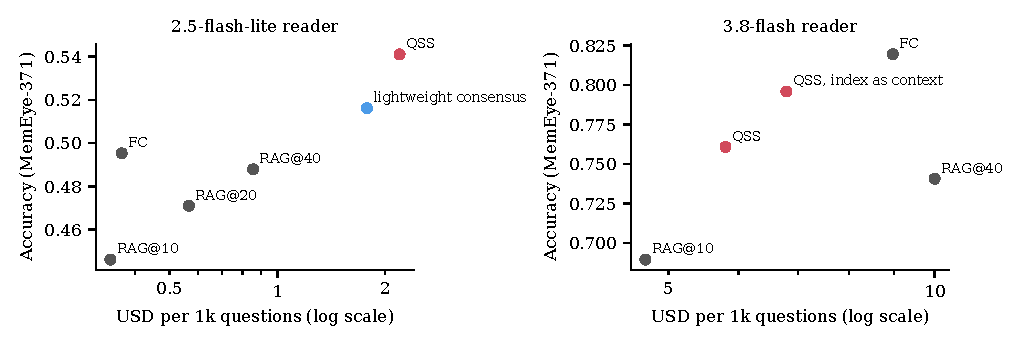
\includegraphics[width=0.92\linewidth]{figures/cost.pdf}
\caption{End-to-end accuracy versus inference cost per 1,000 MemEye questions (logarithmic scale) for the lightweight reader without thinking (left) and the strong reader (right). Points for \qss{} reflect warm-cache cost estimates for persistent user indices; all baseline points reflect measured costs.}
\label{fig:cost}
\end{figure}

The results in Table~\ref{tab:e2e} and Figure~\ref{fig:cost} highlight four key patterns. First, for the lightweight reader without thinking, \qss{} reaches 0.541 accuracy, outperforming both RAG@40 ($+0.053$ $[+0.009, +0.098]$) and full-context reading ($+0.046$ $[+0.001, +0.092]$) while matching the accuracy achieved on oracle annotated evidence (0.539); when the lightweight reader is given a 1,024-token thinking budget, \qss{} similarly improves over RAG@40 by $+0.045$ $[+0.003, +0.086]$ (Wilcoxon $p{=}0.031$ across scenarios). Crucially, the lightweight reader requires an evidence set that is simultaneously complete and concise: the dynamic cutoff control ($S_{\mathrm{grade}}$) opens too few rounds and trails \qss{} by $-0.032$ $[-0.065, -0.001]$, whereas taking the union of \qss{} and cosine top-20 increases FSR to 0.973 (22.4 rounds) but reduces accuracy by $-0.069$ $[-0.111, -0.027]$ because the extra distractor rounds impair lightweight reading. Second, for the strong reader, providing the selected rounds alone yields a modest $+0.020$ over RAG@40, but prepending the text index as narrative context (\qss{}, index as context) raises accuracy to 0.796—a gain of $+0.055$ $[+0.021, +0.089]$ over RAG@40 that remains statistically significant under two-stage scenario-level bootstrap ($[+0.004, +0.126]$, Wilcoxon $p{=}0.031$) and comes within 0.024 of full-context reading while inspecting 7.3 instead of 126.5 image rounds. This contrast arises because the strong reader leverages the global timeline in the index to anchor relative references, whereas the lightweight reader is distracted by the extra index text ($-0.019$). Third, all rankings are preserved under the independent Qwen3-VL-235B-A22B judge, where \qss{} beats RAG@40 by $+0.057$ $[+0.012, +0.102]$ with the lightweight reader and $+0.044$ $[+0.012, +0.080]$ with the strong reader plus index context (Appendix~\ref{app:results}). Fourth, on MemEye+1k (4,088.5 rounds, Appendix Table~\ref{tab:robust}), full-context accuracy with the lightweight reader collapses from 0.495 to 0.368, whereas \qss{} maintains 0.538 ($+0.067$ $[+0.024, +0.111]$ over RAG@40 and $+0.170$ over full context); on Mem-Gallery, \qss{} improves the lightweight reader by $+0.035$ $[+0.015, +0.056]$ over full context. Under a warm prefix cache, \qss{} with index context for the strong reader costs \$6.80 per 1,000 queries, compared to \$10.00 for RAG@40 (whose per-query retrieved rounds cannot be cached across queries).

In summary, RQ2 confirms that resolving compact, complete evidence sets significantly improves end-to-end answering on high-visibility multimodal memory. Lightweight readers benefit directly from distractor-free evidence sets especially as history length scales, while strong readers achieve near-full-context accuracy at lower cost when selected rounds are paired with the global index.

\subsection{RQ3: Generalization to Low-Visibility Histories and the Index Visibility Boundary}
\label{sec:rq3}

To examine how frozen \qss{} generalizes to conversational histories with a fundamentally different discourse structure, we evaluate the exact index configuration and prompts developed on MemEye directly on held-out MemLens at 32k (699 queries for the lightweight reader; 200 queries for the strong reader) and 128k (200 queries for the lightweight reader). Table~\ref{tab:memlens} presents end-to-end accuracy under the official MemLens judge, paired differences relative to RAG@40, mean opened rounds, and measured cost.

\begin{table}[t]
\centering
\caption{Held-out end-to-end accuracy on MemLens under the official benchmark judge (Qwen3-VL-235B-A22B; re-scoring with \texttt{gemini-3.8-flash} yields 96--97\% agreement). $\Delta$ reports paired differences relative to RAG@40 with 95\% bootstrap confidence intervals. Because MemLens assigns an independent haystack to each question, all reported costs are uncached.}
\label{tab:memlens}
\small
\begin{tabular}{llrccr}
\toprule
Setting & Method & Rounds & Accuracy & $\Delta$ vs.\ RAG@40 & \$ / 1k q \\
\midrule
\multirow{11}{*}{\shortstack[l]{32k, 2.5-flash-lite\\(699 questions)}}
 & Full context (FC) & 64.6 & 0.454 & $-0.020$ $[-0.046, +0.004]$ & 3.06 \\
 & RAG@20 & 20.0 & 0.458 & $-0.016$ & 0.79 \\
 & RAG@40 & 40.0 & 0.474 & -- & 1.74 \\
 & Annotated evidence & 5.9 & 0.496 & $+0.023$ $[-0.007, +0.053]$ & 0.46 \\
 & \qss{}, frozen 200-character index & 6.1 & 0.484 & $+0.010$ $[-0.020, +0.040]$ & 6.84 \\
 & \qss{}, 600-character index & 3.9 & \textbf{0.502} & $+0.029$ $[-0.001, +0.059]$ & 8.36 \\
 & Dynamic cutoff control ($S_{\mathrm{grade}}$) & 3.4 & 0.474 & $+0.000$ $[-0.033, +0.031]$ & 10.89 \\
 & Lightweight selector, sampling consensus & 6.4 & 0.448 & $-0.026$ $[-0.056, +0.003]$ & 1.26 \\
 & Qwen3-235B-A22B selector, same prompt & 1.4 & 0.313 & $-0.160$ $[-0.197, -0.124]$ & 0.96 \\
 & \texttt{gpt-5-mini} selector, same prompt & 7.4 & 0.449 & $-0.024$ $[-0.053, +0.003]$ & 4.08 \\
 & Union of \qss{} and cosine top-20 & 21.5 & 0.474 & $+0.000$ $[-0.024, +0.024]$ & 7.31 \\
\midrule
\multirow{5}{*}{\shortstack[l]{32k, 3.8-flash\\(200 questions)}}
 & Full context (FC) & 64.8 & 0.725 & $-0.030$ $[-0.075, +0.010]$ & 24.98 \\
 & RAG@40 & 40.0 & \textbf{0.755} & -- & 14.83 \\
 & Annotated evidence & 5.8 & 0.730 & $-0.025$ $[-0.070, +0.020]$ & 4.66 \\
 & \qss{}, frozen 200-character index & 6.0 & 0.675 & $-0.080$ $[-0.135, -0.030]$ & 10.70 \\
 & \qss{}, index as context & 6.0 & 0.670 & $-0.085$ $[-0.140, -0.035]$ & 16.16 \\
\midrule
\multirow{4}{*}{\shortstack[l]{128k, 2.5-flash-lite\\(same 200 questions)}}
 & Full context (FC) & 245.0 & 0.440 & $-0.035$ $[-0.100, +0.030]$ & 11.65 \\
 & RAG@40 & 40.0 & 0.475 & -- & 1.16 \\
 & Annotated evidence & 5.8 & 0.500 & $+0.025$ $[-0.040, +0.090]$ & 0.45 \\
 & \qss{}, frozen 200-character index & 6.6 & \textbf{0.505} & $+0.030$ $[-0.030, +0.090]$ & 21.75 \\
\bottomrule
\end{tabular}
\end{table}

Table~\ref{tab:memlens} reveals three diagnostic patterns. First, with the lightweight reader at 32k, frozen 200-character \qss{} reaches 0.484 accuracy, exceeding full-context reading ($0.454$) and matching the dynamic cutoff control ($0.474$) at lower cost, but providing only an insignificant $+0.010$ $[-0.020, +0.040]$ gain over RAG@40 ($0.474$); at 128k, frozen \qss{} reaches 0.505 ($\Delta = +0.030$ $[-0.030, +0.090]$ over RAG@40 and $+0.065$ $[+0.010, +0.120]$ over full context). Stratifying by question type (Appendix Table~\ref{tab:memlens_type}) shows that frozen \qss{} outperforms RAG@40 on multi-session reasoning ($0.252$ versus $0.189$) and information extraction ($0.626$ versus $0.598$), but lags on temporal reasoning and knowledge updates. Widening the index snippet from 200 to 600 characters lifts lightweight reader accuracy to 0.502 ($\Delta = +0.029$ $[-0.001, +0.059]$ over RAG@40), surpassing even oracle annotated evidence ($0.496$). Second, with the strong reader, frozen \qss{} scores 0.675, falling $-0.080$ $[-0.135, -0.030]$ below RAG@40 ($0.755$). Notably, even oracle annotated evidence scores $0.730 < 0.755$ with the strong reader, demonstrating that MemLens annotations omit surrounding session turns that a strong reader actively exploits when given 40 rounds. Third, measuring ground-truth index visibility $v(q)$ (Equation~\eqref{eq:vis}) explains the structural divergence between MemEye and MemLens: on MemEye, where user messages have a median length of 45 characters and directly discuss the shared image, $v(q)$ is $0.95$; on MemLens, where gold user messages have a median length of 532 characters and crucial facts or visual references appear as incidental remarks late in the turn, $v(q)$ under a 200-character snippet drops to $0.37$. Widening the snippet to 600 characters raises MemLens index visibility to $0.63$, but also reveals a second bottleneck: even given complete oracle evidence, the lightweight reader achieves only 0.496 overall on MemLens.

Together, RQ3 establishes the exact operating boundary of plain index selection. While \qss{} consistently beats equal-size cosine retrieval in set recall, a 200-character index hides the majority of evidence terms in long multi-topic turns ($v{=}0.37$), and lightweight readers remain bottlenecked by multi-round aggregation even when the relevant rounds are retrieved—directly motivating Visibility-Gated Set Reading (VGS), which we evaluate next.

\subsection{RQ4: Effectiveness of Visibility-Gated Set Reading on Held-Out Data}
\label{sec:rq4}

To verify whether VGS resolves both low index visibility and the lightweight reader aggregation bottleneck, we first compare candidate mechanisms on the development data (all 371 MemEye questions and the 233-question MemLens development split) and then evaluate the frozen VGS pipeline once on the held-out 466-question MemLens test split. Table~\ref{tab:p5dev} summarizes the development mechanisms with the lightweight reader, and Table~\ref{tab:p5test} reports the held-out test results across both readers, including an ablation that replaces \qss{} with cosine top-20 on the low-visibility path (VGS-cheap) and a variant applying the widened index to the strong reader without notes (VGS-strong).

\begin{table}[t]
\centering
\caption{Mechanism ablations on development data with the lightweight reader (\texttt{gemini-2.5-flash-lite}): MemEye (371 questions) and the MemLens development split (233 questions). Per-member notes are generated per selected round by \texttt{gemini-2.5-flash-lite}; cost reflects measured expenditure per 1,000 MemLens questions.}
\label{tab:p5dev}
\small
\begin{tabular}{lccr}
\toprule
Mechanism & MemEye & MemLens dev & \$ / 1k q \\
\midrule
RAG@40 & 0.488 & 0.489 & 1.77 \\
RAG@40 with a 1,024-token thinking budget & \textbf{0.552} & 0.515 & 1.99 \\
\qss{}, 200-character index lines & 0.541 & 0.485 & 6.83 \\
\quad + session closure (all rounds of selected sessions) & 0.526 & 0.476 & 7.21 \\
\qss{}, model-written gist instead of verbatim snippet & 0.504 & 0.515 & 7.15 \\
\qss{}, 600-character index lines & 0.528 & 0.549 & 8.32 \\
\quad + session closure & -- & 0.472 & 8.86 \\
\quad + per-member evidence notes & 0.517 & \textbf{0.562} & 8.83 \\
Cosine top-20 + per-member evidence notes & 0.471 & 0.536 & 2.47 \\
Sentence-granular cosine top-20 & -- & 0.489 & 0.97 \\
VGS (visibility gate $\tau{=}0.7$) & 0.541 & 0.558 & 8.60 \\
\bottomrule
\end{tabular}
\end{table}

\begin{table}[t]
\centering
\caption{Held-out evaluation of VGS on the MemLens test split (466 questions; official judge). $\Delta$ reports paired differences relative to RAG@40 with 95\% bootstrap confidence intervals. VGS-cheap substitutes cosine top-20 with notes on the low-visibility branch; VGS-strong applies the visibility gate to the strong reader without per-member notes.}
\label{tab:p5test}
\small
\begin{tabular}{llccr}
\toprule
Reader & Method & Accuracy & $\Delta$ vs.\ RAG@40 & \$ / 1k q \\
\midrule
\multirow{8}{*}{2.5-flash-lite}
 & RAG@40 & 0.466 & -- & 1.73 \\
 & RAG@40 with thinking (1,024 tokens) & 0.496 & $+0.030$ $[-0.013, +0.073]$ & 1.94 \\
 & \qss{}, 200-character index lines & 0.483 & $+0.017$ $[-0.019, +0.054]$ & 6.84 \\
 & \qss{}, 600-character index lines & 0.479 & $+0.013$ $[-0.024, +0.049]$ & 8.38 \\
 & \qss{}, 600-character lines + per-member notes & 0.536 & $+0.071$ $[+0.032, +0.109]$ & 8.88 \\
 & Cosine top-20 + per-member notes & 0.485 & $+0.019$ $[-0.019, +0.058]$ & 2.50 \\
 & VGS ($\tau{=}0.7$) & \textbf{0.536} & $+0.071$ $[+0.032, +0.109]$ & 8.63 \\
 & VGS-cheap & 0.494 & $+0.028$ $[-0.011, +0.069]$ & 3.08 \\
\midrule
\multirow{4}{*}{3.8-flash}
 & RAG@40 & \textbf{0.689} & -- & 14.74 \\
 & \qss{}, 200-character index lines & 0.618 & $-0.071$ $[-0.107, -0.034]$ & 10.79 \\
 & \qss{}, 600-character index lines & 0.659 & $-0.030$ $[-0.062, +0.002]$ & 11.35 \\
 & VGS-strong & 0.655 & $-0.034$ $[-0.069, -0.002]$ & 11.21 \\
\bottomrule
\end{tabular}
\end{table}

Tables~\ref{tab:p5dev} and~\ref{tab:p5test} establish four central findings. First, diagnostic analysis on the development data confirms that lightweight readers are bottlenecked by set aggregation rather than set recall alone: given complete oracle evidence on MemLens, \texttt{gemini-2.5-flash-lite} answers only 6\% of arithmetic queries and 9\% of counting queries (versus 67\% and 91\% for \texttt{gemini-3.8-flash}), and on MemEye its accuracy on complete \qss{} sets drops from 0.64 ($|G|{=}1$) to 0.45 ($|G|\ge 4$). Consequently, naively expanding the selected set via session closure (appending all rounds from any selected session) increases MemLens development FSR from 0.292 to 0.824 but reduces accuracy from 0.549 to 0.472 (and from 0.541 to 0.526 on MemEye) by introducing distracting turns; replacing verbatim snippets with model-written gists also hurts MemEye (0.504 versus 0.541) by stripping exact phrasing. Second, on the held-out MemLens test split (Table~\ref{tab:p5test}), VGS achieves 0.536 accuracy with the lightweight reader, outperforming RAG@40 ($0.466$) by $+0.071$ $[+0.032, +0.109]$ and RAG@40 with thinking ($0.496$) by $+0.041$ $[-0.002, +0.084]$. Comparing rows within Table~\ref{tab:p5test} isolates the source of this improvement: widening index lines to 600 characters alone yields only $+0.013$ on the test split, whereas adding per-member evidence notes over the exact same 600-character \qss{} selections adds $+0.058$ $[+0.021, +0.097]$. At the same time, generating notes over a noisy cosine top-20 pool yields only $+0.019$ ($0.485$), demonstrating that per-member notes require the compact, high-precision sets produced by \qss{}. Third, breaking down the held-out test gains by question subtype shows that VGS specifically remedies multi-item aggregation failures: accuracy rises from 0.03 to 0.21 on arithmetic, from 0.10 to 0.23 on counting, and from 0.12 to 0.38 on temporal ordering. Fourth, the label-free visibility gate $\hat{v}(q) \ge 0.7$ accurately separates benchmark regimes without supervision: it routes 98.7\% of MemEye queries and 87.7\% of Mem-Gallery queries to the high-visibility path—preserving the full 0.541 accuracy on MemEye (where un-gated notes lower accuracy to 0.517) and 0.852 on Mem-Gallery—while routing 87.6\% of MemLens queries to the low-visibility path. For the strong reader, widening the index narrows the gap to RAG@40 from $-0.071$ to $-0.030$ $[-0.062, +0.002]$ at 23\% lower cost (\$11.35 versus \$14.74), though RAG@40 remains highest ($0.689$) because the strong reader natively aggregates 40 raw rounds.

Overall, RQ4 demonstrates that VGS successfully turns index visibility into an actionable query-time control mechanism. For lightweight readers, pairing widened index selection with explicit per-member evidence notes yields a $+0.071$ held-out improvement over wide retrieval without degrading performance on high-visibility histories.

\subsection{RQ5: Locus of Selection Capability and Lightweight Amortization}
\label{sec:rq5}

To understand why \qss{} achieves high full-set recall and whether this capability can be shifted to write time, elicited from lightweight models via prompting, or transferred zero-shot across model families, we conduct systematic selection ablations on MemEye. Table~\ref{tab:ablate} reports the mean number of opened rounds and Full-Set Recall across four categories of interventions: varying the selector model under a fixed prompt and index, injecting write-time organization created by the strong model at ingestion, applying structural prompting strategies to the lightweight selector (\texttt{gemini-2.5-flash-lite}), and applying our two lightweight amortization mechanisms (sampling consensus and online resolution write-back).

\begin{table}[t]
\centering
\caption{Ablation study on the locus of set-selection capability (MemEye, selection only). Values in brackets give the FSR of cosine retrieval at the same per-question size when $|S(q)|$ differs substantially from baseline. Rows marked $^\ddagger$ are evaluated on a fixed random subset of 150 questions (where \texttt{gemini-3.8-flash} achieves 0.887 FSR in 7.7 rounds). The baseline lightweight selector (\texttt{gemini-2.5-flash-lite}) achieves 0.712 FSR in 9.8 rounds.}
\label{tab:ablate}
\small
\resizebox{\linewidth}{!}{%
\begin{tabular}{llrc}
\toprule
Category & Intervention & Rounds & FSR \\
\midrule
\multirow{7}{*}{\shortstack[l]{Selector model\\(same prompt and index)}}
 & \texttt{gemini-3.8-flash} (\qss{}) & 7.3 & 0.903 \\
 & \texttt{gemini-3.5-flash-lite} / \texttt{gemini-3.1-flash-lite} & 3.9 / 4.3 & 0.685 / 0.660 \\
 & \texttt{gemini-2.5-flash-lite}, without / with a 2,048-token thinking budget & 9.8 / 4.6 & 0.712 / 0.636 \\
 & \texttt{gpt-5-mini} & 5.9 & 0.728 \\
 & \texttt{gpt-5}$^\ddagger$ & 2.8 & 0.573 \\
 & Qwen3-235B-A22B, thinking$^\ddagger$ & 2.3 & 0.407 \\
 & Qwen3-235B-A22B, instruction & 1.5 & 0.264 \\
\midrule
\multirow{3}{*}{\shortstack[l]{Write-time organization\\(strong model at ingestion)}}
 & Static named groups written once; lightweight selector picks groups (+ cosine top-5) & 22.1 (23.2) & 0.636 (0.717) \\
 & Predicted discourse aliases appended to index; lightweight selector & 9.3 & 0.736 \\
 & Predicted discourse aliases appended to cosine keys (top-10 / top-40) & 10 / 40 & 0.642 / 0.933 \\
\midrule
\multirow{5}{*}{\shortstack[l]{Prompting and structure\\(lightweight selector)}}
 & Predict group cardinality first, then enumerate member rounds & 8.1 & 0.663 \\
 & Decompose query into membership predicates and verify per predicate & 8.7 & 0.617 \\
 & Add explicit narrative coordinates and session headers to index & 10.0 & 0.690 \\
 & In-context distillation with three strong-selector demonstrations & 8.8 & 0.639 \\
 & Chunked exhaustive scan (30 rounds per call) & 18.4 & 0.765 [0.782] \\
\midrule
\multirow{4}{*}{\shortstack[l]{Lightweight amortization\\(lightweight selector)}}
 & Union of $K{=}5$ sampled selections ($V{=}1$) / consensus ($V{=}2$) & 15.2 / 10.7 & 0.836 [0.714] / 0.749 \\
 & Online resolution write-back using resolutions produced by the lightweight selector itself & 9.7 & 0.725 \\
 & Online resolution write-back using strong resolutions for 30\% / 100\% of prior queries & 9.5 / 9.5 & 0.741 / 0.752 \\
 & Model-free reuse of top-3 nearest resolved sets + cosine top-5 & 19.1 & 0.836 [0.787] \\
\bottomrule
\end{tabular}}
\end{table}

Table~\ref{tab:ablate} reveals four insights into how set selection operates. First, query-time set resolution cannot be replaced by static write-time organization even when the strong model performs the write-time processing: having \texttt{gemini-3.8-flash} partition each history into named topical groups at ingestion yields 22.1 rounds but only 0.636 FSR because user queries define cross-cutting sets that span multiple sessions, and augmenting rounds with write-time predicted aliases barely moves cosine top-10 recall (0.633 to 0.642) or lightweight selection (0.712 to 0.736). Second, structural prompting interventions do not close the gap for the lightweight selector: two-step cardinality-then-member prompting (0.663), predicate decomposition (0.617), narrative session coordinates (0.690), and few-shot demonstrations from strong selections (0.639) all perform at or below the unaided lightweight baseline (0.712), while allocating a 2,048-token thinking budget makes the lightweight model overly conservative (opening 4.6 rounds at 0.636 FSR). Error inspection shows that unaided lightweight failures stem primarily from selecting wrong members rather than too few: on failed queries, \texttt{gemini-2.5-flash-lite} opens 11.1 rounds for 4.3 gold rounds. Third, zero-shot cross-family evaluation under the uncalibrated Gemini prompt shows that recall calibration varies sharply by model family rather than model scale: \texttt{gpt-5-mini} achieves 0.728 FSR on MemEye (and 0.442 on MemLens, outperforming \texttt{gemini-3.8-flash} at 0.375), whereas larger or reasoning-tuned models (\texttt{gpt-5} and Qwen3-235B-A22B) default to high-precision, small-cardinality outputs (1.5--2.8 rounds), sacrificing full-set recall when not calibrated for inclusive selection. Finally, our two amortization mechanisms recover a substantial fraction of the lightweight gap at minimal cost: sampling consensus ($K{=}5, V{=}2$) raises FSR from 0.712 to 0.749 in 10.7 rounds, and online resolution write-back reaches 0.752 FSR when reusing prior strong resolutions (or 0.741 when only 30\% of prior queries are resolved by the strong selector, and 0.806 FSR when combined with sampling consensus, lifting end-to-end accuracy to 0.518 in Table~\ref{tab:e2e}).

These ablations establish that resolving multimodal evidence sets is fundamentally a query-time reasoning operation that requires family-specific recall calibration; it cannot be pre-computed into static write-time clusters, but can be partially amortized over time as the memory accumulates resolved query sets.

\subsection{RQ6: Visual Granularity: Reader-Driven Zooming and Write-Time Captions}
\label{sec:rq6}

To investigate whether fine-grained visual perception rather than set-level localization limits multimodal memory performance, we evaluate two widely proposed visual enhancements on MemEye: two-pass reader-driven image zooming and write-time dense captioning. Under the zooming protocol, the reader first inspects the multimodal context at standard resolution and requests up to three high-resolution bounding-box crops (each specified by an image identifier and normalized coordinates), and then answers in a second pass where the baseline prompt is augmented with the requested crops (or upgraded in place). We compare voluntary reader-chosen zooming against forced zooming (requiring 1--3 crops) and a blind zoom control (automatically adding three fixed tiles of the single image most similar to the query), with full results reported in Appendix Table~\ref{tab:zoom}.

The experimental results show that neither reader-driven zooming nor dense caption replacement provides reliable gains over reading original images at standard resolution. First, for the strong reader (\texttt{gemini-3.8-flash}) in full context, voluntary reader-chosen zooming triggers crop requests on 246 of the 371 questions and significantly lowers overall accuracy from 0.819 to 0.790 ($\Delta = -0.029$ $[-0.056, -0.002]$), while upgrading the selected images to high resolution in place yields $0.803$ ($\Delta = -0.017$ $[-0.042, +0.009]$). For the lightweight reader (\texttt{gemini-2.5-flash-lite}) on oracle annotated evidence, voluntary zooming ($0.552$) and forced zooming ($0.551$) fail to exceed the heuristic blind zoom control ($0.561$ versus $0.539$ without zoom), indicating that the slight gain comes from supplying additional image tokens rather than accurate region localization; only on multi-image \qss{} sets (7.3 rounds) does forced zooming ($0.557$) outperform blind zooming ($0.523$). Second, substituting write-time dense captions for original images degrades full-context accuracy for both the strong reader ($0.779$ versus $0.819$) and the lightweight reader ($0.474$ versus $0.495$), and appending dense captions alongside original images in \qss{} sets reduces lightweight reader accuracy from $0.541$ to $0.526$.

Together, RQ6 confirms that on current multimodal memory benchmarks, pixel resolution is rarely the primary bottleneck once original images are preserved: low-resolution images already suffice for global perception, and localized zooming cannot substitute for retrieving the complete set of relevant rounds.

\section{Related Work}
\label{sec:related}

\paragraph{Memory construction versus raw-history retrieval.} Conversational memory architectures differ fundamentally in how much computation and compression they apply at write time versus query time. Early agent frameworks score raw memory streams by recency, importance, and embedding similarity~\citep{park2023generative} or page context between storage tiers via tool calls~\citep{packer2023memgpt}, whereas structured memory systems such as Mem0~\citep{chhikara2025mem0} and A-MEM~\citep{xu2025amem} extract, consolidate, and link atomic memory notes at ingestion. Recent controlled evaluations challenge the necessity of write-time rewriting in text memory: retrieving raw dialogue turns via dense embeddings matches or outperforms explicit memory systems across LoCoMo, LongMemEval, and related benchmarks~\citep{bao2026rawrag,zhou2026explicit}, single-call LLM turn selection replaces fact extraction under tight token budgets~\citep{sharma2026selection}, and explicit memory extraction primarily acts as a costly scaffold for weak readers~\citep{peng2026memorytax}. Our study confirms the large-budget sufficiency of raw retrieval in text memory, identifies set completeness and the cross-modal embedding gap as the exact points where top-$k$ similarity fails in multimodal memory, and demonstrates how query-time set selection and visibility-gated reading address these failures without lossy write-time compression.

\paragraph{Multimodal agent memory benchmarks.} Recent benchmarks extend long-term conversational memory to visual inputs with varying degrees of visual necessity and discourse complexity. MemEye~\citep{guo2026memeye} curates multi-session life logs in which questions require synthesizing visual details across sessions, and Mem-Gallery~\citep{bei2026memgallery} evaluates multimodal memory across 20 conversational scenarios. MemLens~\citep{ren2026memlens} pairs multi-session dialogues with needle images whose removal drops frontier VLM accuracy below 2\%, showing that long-context models degrade with distraction while storage-time memory compression loses visual fidelity. In parallel, LongMemEval-V2~\citep{wu2026lmev2} evaluates trajectory memory with screenshots for web agents and finds that an agentic file explorer outperforms dense RAG, while Visual Haystacks~\citep{wu2025visualhaystacks} studies multi-needle retrieval in large image collections. Our cross-benchmark analysis bridges these efforts by introducing index visibility and visual ablation survival as quantitative properties that explain why a retrieval mechanism succeeds on concise, image-foregrounded logs (MemEye) yet requires visibility gating on long, multi-topic conversations (MemLens).

\paragraph{Index-based navigation and LLM reranking.} Operating over a compact index before inspecting primary content is a classic paradigm in long-context processing. ReadAgent compresses long documents into episode gists and looks up raw pages on demand~\citep{lee2024readagent}, and MemWalker traverses a hierarchical summary tree~\citep{chen2023memwalker}. In information retrieval, LLMs are widely deployed as listwise rerankers~\citep{sun2023rankgpt} or fine-grained relevance graders~\citep{zhuang2024beyond}, while Adaptive-RAG routes queries across retrieval depths based on predicted query complexity~\citep{jeong2024adaptiverag}. \qss{} and VGS advance this line of work in three ways: first, our same-model controls ($S_{\mathrm{rank}}$ and $S_{\mathrm{grade}}$) prove that formulating retrieval as unordered set resolution with adaptive cardinality adds significant full-set recall beyond listwise ranking and graded relevance cutoffs; second, VGS introduces a zero-cost, label-free estimator of index visibility $\hat{v}(q)$ that gates both index horizon and per-member evidence note extraction; and third, our cross-family experiments reveal that set cardinality calibration is highly sensitive to model family and prompt tuning rather than raw model scale.

\paragraph{Set-level recall, write-time organization, and experiential write-back.} Evaluating retrieval by complete evidence sets connects agent memory to multi-hop question answering~\citep{yang2018hotpotqa}, multi-hop passage all-recall~\citep{gutierrez2024hipporag}, and high-recall technology-assisted review~\citep{cormack2015autonomy}. Whereas corpus-level methods such as GraphRAG~\citep{edge2024graphrag}, RAPTOR~\citep{sarthi2024raptor}, HippoRAG~\citep{gutierrez2024hipporag}, and Doc2Query~\citep{nogueira2019doc2query} reorganize or expand documents at indexing time, our ablations show that static write-time groups and predicted aliases fail to capture personal memory sets defined dynamically by user queries. Instead, our online resolution write-back mechanism learns at test time from answered queries—analogous to how MemPrompt stores user feedback for misunderstood intents~\citep{madaan2022memprompt} and ExpeL accumulates cross-task execution insights~\citep{zhao2024expel}—by recording resolved evidence sets directly into the user index to amortize future set selection.

\section{Discussion}
\label{sec:discussion}

\paragraph{Operating regimes of multimodal agent memory.} Synthesizing results across all five benchmarks reveals that multimodal memory performance is governed by the interaction of three measurable factors: set structure, index visibility, and reader aggregation capacity. First, when queries target single items or when conversational text redundantly describes the images (as in Mem-Gallery, where removing all visual inputs still leaves 0.892 accuracy), wide cosine retrieval (RAG@40) already recovers the necessary context. Second, when queries target multi-round visual sets and the compact index exposes the relevant cues ($\hat{v}(q) \ge \tau$, as in MemEye where $v{=}0.95$), \qss{} resolves complete sets in roughly 7 rounds, improving accuracy for both lightweight readers (by eliminating distractor rounds) and strong readers (when paired with the index as global narrative context). Third, when evidence is buried inside long multi-topic messages ($\hat{v}(q) < \tau$, as in MemLens where $v{=}0.37$), reader capacity dictates the optimal strategy: strong readers (\texttt{gemini-3.8-flash}) natively aggregate across 40 raw rounds and exploit unannotated contextual turns, making wide similarity retrieval (RAG@40) their strongest option; lightweight readers (\texttt{gemini-2.5-flash-lite}), however, cannot aggregate raw sets even when retrieval is complete, and require the widened index and explicit per-member evidence notes provided by VGS.

\paragraph{Role separation between write time and query time.} A consistent empirical principle emerging from our study is that write-time operations should construct navigation keys, never replace perception or pre-commit to static set boundaries. Whenever write-time outputs replaced raw multimodal content—such as substituting dense or short captions for original images, or replacing verbatim message snippets with model-written gists—end-to-end accuracy declined because query-specific visual details and exact lexical cues were lost. Similarly, static write-time clustering failed because user queries slice personal histories along ad-hoc dimensions (e.g., comparing two specific days or tracking a recurring object across unrelated sessions). Conversely, write-time artifacts were indispensable as lightweight navigation keys: short captions bridged the embedding modality gap during cosine prefiltering (lifting coverage@10 from 0.300 to 0.774), and append-only index lines enabled prefix-cached query-time navigation. The only write-back operation that improved set selection was online resolution write-back, which records query-time set resolutions after they occur rather than guessing them at ingestion.

\paragraph{Allocating model capability and calibrating cross-family selectors.} Because \qss{} processes only compact text index lines whose prefix remains static across queries, spending strong-model compute on query-time navigation is highly economical in persistent per-user deployments: under a warm prefix cache, strong selection plus strong reading with index context on MemEye costs \$6.80 per 1,000 queries, compared to \$10.00 for RAG@40. At the same time, our cross-family evaluations demonstrate that set selection quality does not scale monotonically with general model size or reasoning capability. Under a fixed prompt, \texttt{gpt-5} and Qwen3-235B-A22B returned overly conservative sets of 1.4 to 2.8 rounds, whereas \texttt{gpt-5-mini} opened 5.9 to 7.4 rounds and achieved the highest full-set recall on MemLens (0.442). Instruction-tuned and reasoning models exhibit a strong prior toward precision that overrides generic instructions to be inclusive; deploying \qss{} with a new model family therefore requires calibrating the selector prompt on development queries to verify that the mean cardinality $|S(q)|$ matches the expected set size.

\paragraph{Methodological implications for benchmark evaluation.} Our findings carry three implications for how multimodal memory benchmarks should be evaluated. First, item-level recall@$k$ and coverage conceal catastrophic failures on multi-item queries; reporting Full-Set Recall ($\mathrm{FSR}$) alongside the number of opened rounds $|S(q)|$ is essential for evaluating set-level retrieval. Second, reporting two zero-cost diagnostic metrics—index visibility $v$ and visual ablation accuracy (performance when all images and captions are removed)—immediately situates a benchmark within the design space, distinguishing visually grounded concise logs (MemEye: $v{=}0.95$, visual ablation $0.191$) from visually grounded long-turn logs (MemLens: $v{=}0.37$, visual ablation $<0.02$) and text-redundant logs (Mem-Gallery: visual ablation $0.892$). Third, for benchmarks constructed from a small number of shared scenario histories such as MemEye (8 histories), question-level bootstrap intervals overstate statistical certainty; reporting two-stage scenario-level bootstrap intervals is necessary to distinguish scenario-wide improvements from history-specific fluctuations.

\section{Limitations}
\label{sec:limitations}

Several scope boundaries should be considered when interpreting our results. First, while MemLens provides 699 independent conversation haystacks, MemEye comprises eight shared scenario histories; under two-stage scenario-level bootstrap on MemEye (Appendix Table~\ref{tab:cluster}), the retrieval gains of \qss{} (8 of 8 scenarios positive, $p{=}0.008$), the end-to-end gain of the strong reader with index context ($p{=}0.031$), and the gain of the lightweight reader with thinking ($p{=}0.031$) remain statistically significant, whereas the interval for the non-thinking lightweight reader spans zero ($[-0.014, +0.120]$, 6 of 8 scenarios positive). Second, because MemEye and MemLens differ simultaneously in message length, discourse style, and annotation granularity, index visibility $v(q)$ is an observational property that explains cross-benchmark variance and guides VGS routing, rather than an isolated causal variable manipulated within a single synthetic corpus; moreover, because MemLens gold sets are derived from session-level annotations and turn flags, strong readers can benefit from unflagged session turns, making $\mathrm{FSR}$ a conservative proxy on that benchmark. Third, our cross-family selector comparisons evaluate a single prompt developed with \texttt{gemini-3.8-flash} without per-family prompt tuning, and thus measure zero-shot prompt transferability rather than the upper bound of other model families. Fourth, our scale experiment (MemEye+1k) interleaves distractor sessions from different users in Mem-Gallery, which are easier to separate semantically than long-term distractors generated by the same user on overlapping topics. Finally, warm-cache cost estimates assume a persistent per-user index with high cache hit rates, whereas benchmarks with independent per-question haystacks (such as MemLens) incur uncached selection costs unless amortized over multi-turn user sessions.

\section{Conclusion}
\label{sec:conclusion}

We investigated what remains unsolved in agent memory when raw similarity retrieval already matches dedicated memory systems on text benchmarks. While large-budget cosine retrieval suffices for text conversations, multimodal agent memory frequently requires resolving complete sets of historical rounds linked by narrative aliases and aggregating visual facts across them—tasks where independent top-$k$ similarity and write-time compression break down. We introduced a unified framework pairing Query-Time Set Selection (\qss{}), which resolves variable-size evidence sets over an append-only, prefix-cacheable text index while preserving raw images for perception, with Visibility-Gated Set Reading (VGS), which estimates index visibility without labels at query time to adapt index horizons and generate explicit per-member evidence notes when evidence is buried in long turns. Across five benchmarks, same-model controls confirm that the set formulation adds substantial full-set recall over listwise ranking and dynamic relevance cutoffs, while VGS delivers a $+0.071$ end-to-end improvement for lightweight readers on held-out low-visibility data without sacrificing efficiency or accuracy on high-visibility histories. Future work should explore query-adaptive index construction that dynamically expands long turns without full re-indexing, as well as lightweight selector fine-tuning to internalize inclusive set calibration across model families.

\bibliographystyle{plainnat}
\bibliography{refs}

\appendix

\section{Prompts and Evaluation Rubrics}
\label{app:prompts}

\paragraph{Set selector (\qss{}).} Both the primary \qss{} selector and all lightweight selectors receive the following system instruction, followed by the memory index $I(H)$ (or the cosine-prefiltered candidate lines), the optional block of resolved prior queries (when online resolution write-back is active), and the user query $q$. Generation is constrained to the JSON schema \texttt{\{"rounds": [string]\}}:

\begin{quote}\small
You are the retrieval step of a personal assistant's long-term memory. You get a compact index of the user's entire conversation history (one line per round; images are summarised in a few words) and a question. Choose the rounds that must be opened in full (with their original images) to answer the question. Include EVERY round that may hold needed evidence, especially ALL members of any group the question refers to (e.g. all ads of a brand, every scene of an episode, all versions of a screen over time), not just the best match. Include rounds that define labels the question uses (episode/arc names, `first', `later', `updated'). Image summaries are lossy: when unsure whether an image is relevant, include it. Order by importance. Return JSON with the key ``rounds'' and at most 40 ids.
\end{quote}

\paragraph{Same-model controls.} The listwise ranking control ($S_{\mathrm{rank}}$) receives the identical candidate index lines with the instruction to order all candidate rounds from most to least useful for answering the query and return the ordered list of identifiers. The dynamic graded cutoff control ($S_{\mathrm{grade}}$) receives the identical candidate lines with the instruction to grade every candidate round from $0$ (not relevant) to $3$ (contains needed evidence) in a JSON map from round identifiers to integer grades; rounds assigned grade $2$ or $3$ are retained. Cross-family selectors are invoked via OpenRouter using the exact same selector instruction and JSON schema.

\paragraph{Online resolution write-back.} When resolution write-back is enabled, previously resolved queries for the same user history are appended below the index as compact lines pairing the earlier query text with its selected round identifiers, preceded by the header: ``Resolved earlier questions from this user (the rounds that were opened to answer them; the labels they use may refer to the same items as the current question)''.

\paragraph{Reader and per-member evidence notes.} All retrieval conditions evaluated with the same reader share a single answering system instruction. The instruction directs the reader to ground every claim in the provided conversation rounds and images, to prioritize the most recent evidence when facts evolve over time, to inspect visual details carefully, to state explicitly when required information is absent, to refer to visual items using the phrasing established in the dialogue rather than internal round identifiers, and to answer concisely. Because the instruction is held strictly constant across all methods, any phrasing examples within the prompt affect all baselines and proposed methods identically; sensitivity checks excluding the two MemEye questions whose reference answers overlap with an example phrase in the reader instruction alter paired differences between \qss{} and RAG@40 by at most $0.001$ ($+0.054$ $[+0.009, +0.098]$ for the lightweight reader and $+0.056$ $[+0.022, +0.090]$ for the strong reader with index context). In the low-visibility pathway of VGS, the lightweight model (\texttt{gemini-2.5-flash-lite}) first processes each selected round $r_i \in S(q)$ individually with the query $q$ to write a short factual note recording the entities, timestamps, and numerical values relevant to $q$; these notes are prepended to the raw rounds $S(q)$ during final reading.

\paragraph{Evaluation judges.} On MemEye and Mem-Gallery, the evaluation judge applies the official five-level MemEye grading rubric ($\{0, 0.25, 0.5, 0.75, 1.0\}$) comparing the model prediction against the ground-truth reference answer and rubric criteria. On MemLens, the evaluation judge uses the official type-specific binary evaluation prompts released by the benchmark authors without modification.

\section{Additional Empirical Results}
\label{app:results}

\paragraph{Scenario-level uncertainty on MemEye.} Because the 371 questions of MemEye are distributed across eight scenario histories, Table~\ref{tab:cluster} compares standard question-level 95\% bootstrap confidence intervals with two-stage cluster bootstrap intervals (resampling the eight scenarios with replacement, followed by questions within each sampled scenario), alongside the fraction of scenarios showing a positive mean difference and a two-sided Wilcoxon signed-rank test across the eight scenario means.

\begin{table}[h]
\centering
\caption{Question-level and scenario-level 95\% bootstrap confidence intervals for the primary MemEye comparisons, along with the number of scenarios (out of 8) exhibiting a positive mean gain and the Wilcoxon signed-rank $p$-value across scenario means.}
\label{tab:cluster}
\small
\resizebox{\linewidth}{!}{%
\begin{tabular}{lcccrr}
\toprule
Comparison & Mean $\Delta$ & Question-level CI & Scenario-level CI & Scenarios $>0$ & Wilcoxon $p$ \\
\midrule
Lightweight reader: \qss{} $-$ RAG@40 & $+0.053$ & $[+0.009, +0.098]$ & $[-0.014, +0.120]$ & 6/8 & 0.078 \\
Lightweight reader (thinking 1,024): \qss{} $-$ RAG@40 & $+0.045$ & $[+0.003, +0.086]$ & $[-0.005, +0.095]$ & 6/8 & 0.031 \\
Lightweight reader: sampling consensus $-$ RAG@40 & $+0.028$ & $[-0.015, +0.071]$ & $[-0.038, +0.093]$ & 5/8 & 0.250 \\
Strong reader: \qss{} with index context $-$ RAG@40 & $+0.055$ & $[+0.021, +0.089]$ & $[+0.004, +0.126]$ & 6/8 & 0.031 \\
Strong reader: \qss{} $-$ RAG@40 & $+0.020$ & $[-0.014, +0.055]$ & $[-0.030, +0.073]$ & 6/8 & 0.219 \\
Strong reader: \qss{} with index context $-$ full context & $-0.024$ & $[-0.050, +0.002]$ & $[-0.061, +0.022]$ & 1/8 & 0.438 \\
FSR: \qss{} $-$ equal-size cosine retrieval & $+0.364$ & $[+0.310, +0.418]$ & $[+0.221, +0.551]$ & 8/8 & 0.008 \\
FSR: \qss{} ($P{=}100$) $-$ listwise ranking control ($S_{\mathrm{rank}}$) & $+0.059$ & $[+0.032, +0.089]$ & $[+0.008, +0.111]$ & 5/8 & 0.062 \\
\bottomrule
\end{tabular}}
\end{table}

\paragraph{Cross-family judge verification on MemEye.} Re-scoring the primary MemEye conditions with an independent vision-language judge from a separate model family (Qwen3-VL-235B-A22B) using the identical rubric yields slightly stricter absolute scores while preserving every pairwise method ordering: for the lightweight reader, \qss{} achieves $0.514$ and oracle annotated evidence achieves $0.520$, outperforming full-context reading ($0.469$) and RAG@40 ($0.457$, paired $\Delta = +0.057$ $[+0.012, +0.102]$); for the strong reader, full-context reading achieves $0.758$, followed by \qss{} with index context ($0.739$, paired $\Delta = +0.044$ $[+0.012, +0.080]$ over RAG@40), plain \qss{} ($0.701$), and RAG@40 ($0.695$).

\paragraph{Scale robustness (MemEye+1k) and external generalization (Mem-Gallery).} Table~\ref{tab:robust} and Figure~\ref{fig:scale} evaluate performance when each MemEye history is expanded 32-fold by interleaving 1,000 distractor images from Mem-Gallery (4,088.5 mean rounds, $\sim 722\text{k}$ tokens) and on the 903-question Mem-Gallery benchmark. On MemEye+1k, full-context reading with the lightweight reader degrades sharply from $0.495$ to $0.368$, whereas \qss{} (using a cosine prefilter of $P{=}200$) maintains $0.538$ accuracy, outperforming RAG@40 by $+0.067$ $[+0.024, +0.111]$ and full-context reading by $+0.170$. On Mem-Gallery, \qss{} with the lightweight reader outperforms full-context reading by $+0.035$ $[+0.015, +0.056]$ ($0.852$ versus $0.817$) and edges out RAG@40 ($0.839$), whereas the strong reader saturates near $0.91$ across all methods because the dialogue text in Mem-Gallery largely describes the visual content (full-context reading without any images or captions still reaches $0.892$ on a 451-question random half of the benchmark).

\begin{table}[h]
\centering
\caption{End-to-end accuracy on MemEye histories enlarged with 1,000 distractor images (MemEye+1k, 371 questions) and on Mem-Gallery (903 questions). On MemEye+1k, \qss{} applies a cosine prefilter of $P{=}200$ rounds. $^\dagger$Evaluated on a fixed 100-question subset.}
\label{tab:robust}
\small
\begin{tabular}{llccccc}
\toprule
Setting & Reader & FC & RAG@20 & RAG@40 & Lightweight selector & \qss{} \\
\midrule
MemEye (original, 126.5 r) & 2.5-flash-lite & 0.495 & 0.471 & 0.488 & 0.516 & \textbf{0.541} \\
MemEye+1k (4,088.5 r) & 2.5-flash-lite & 0.368 & 0.451 & 0.471 & 0.493 & \textbf{0.538} \\
MemEye+1k (4,088.5 r) & 3.8-flash & 0.848$^\dagger$ & -- & 0.730 & -- & 0.764 \\
Mem-Gallery (903 q) & 2.5-flash-lite & 0.817 & -- & 0.839 & 0.839 & \textbf{0.852} \\
Mem-Gallery (903 q) & 3.8-flash & \textbf{0.917} & -- & 0.912 & -- & 0.908 \\
\bottomrule
\end{tabular}
\end{table}

\begin{figure}[h]
\centering
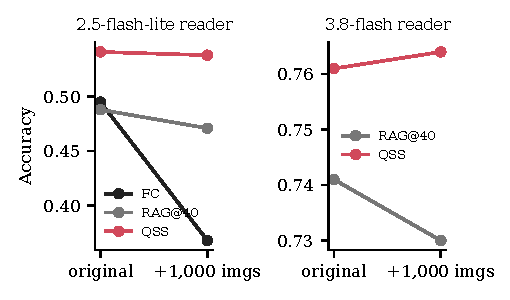
\includegraphics[width=0.5\linewidth]{figures/scale.pdf}
\caption{End-to-end accuracy of full-context reading (FC), RAG@40, and \qss{} on original MemEye histories (126.5 rounds) versus histories enlarged 32-fold with 1,000 distractor images (4,088.5 rounds) for the lightweight reader (left) and the strong reader (right; full context evaluated on the 100-question subset in Table~\ref{tab:robust}).}
\label{fig:scale}
\end{figure}

\paragraph{MemLens breakdown by question category and gold-round definition.} Table~\ref{tab:memlens_type} breaks down the 32k MemLens accuracy of the lightweight reader across the four official question categories. In MemLens, ground-truth annotations specify answer sessions along with turn-level evidence flags for text and separate needle images that often reside in adjacent turns of the same session; we therefore define the ground-truth set $G(q)$ as all rounds within the annotated answer sessions that contain either a flagged evidence turn or a needle image (averaging 5.9 rounds per query, of which 4.1 contain an image).

\begin{table}[h]
\centering
\caption{MemLens-32k accuracy with the lightweight reader (\texttt{gemini-2.5-flash-lite}) stratified by official question category (246, 194, 143, and 116 questions, respectively).}
\label{tab:memlens_type}
\small
\begin{tabular}{lcccc}
\toprule
Method & Information extraction & Temporal reasoning & Multi-session reasoning & Knowledge update \\
\midrule
Full context (FC) & 0.577 & 0.557 & 0.182 & 0.353 \\
RAG@40 & 0.598 & 0.552 & 0.189 & 0.431 \\
Annotated evidence & 0.634 & 0.552 & 0.224 & 0.448 \\
\qss{}, frozen 200-character index & 0.626 & 0.521 & 0.252 & 0.405 \\
\qss{}, 600-character index & 0.634 & 0.577 & 0.266 & 0.388 \\
Dynamic cutoff control ($S_{\mathrm{grade}}$) & 0.630 & 0.505 & 0.203 & 0.422 \\
\bottomrule
\end{tabular}
\end{table}

\paragraph{Reader capacity dependence.} Table~\ref{tab:reader} compares full-context reading, top-$k$ retrieval, and oracle annotated evidence across three readers of decreasing scale on MemEye. While the frontier reader (\texttt{gemini-3.8-flash}) achieves its highest accuracy under full-context reading ($0.819$), both lighter readers (\texttt{gemini-3.1-flash-lite} and \texttt{gemini-2.5-flash-lite}) perform best when given compact, focused evidence sets ($0.694$ and $0.539$, respectively).

\begin{table}[h]
\centering
\caption{End-to-end accuracy on MemEye (371 questions) across three reader models as a function of context selection.}
\label{tab:reader}
\small
\begin{tabular}{lcccc}
\toprule
Reader & Full context & RAG@10 & RAG@40 & Annotated evidence \\
\midrule
\texttt{gemini-3.8-flash} & 0.819 & 0.689 & 0.741 & 0.746 \\
\texttt{gemini-3.1-flash-lite} & 0.639 & 0.601 & 0.612 & 0.694 \\
\texttt{gemini-2.5-flash-lite} & 0.495 & 0.446 & 0.488 & 0.539 \\
\bottomrule
\end{tabular}
\end{table}

\paragraph{Reader-driven zooming and retrieval keys.} Table~\ref{tab:zoom} reports the full matrix of reader-driven zooming experiments from Section~\ref{sec:rq6}, and Table~\ref{tab:keys} reports the gold-evidence coverage@10 across embedding key formulations from Section~\ref{sec:prelim}. Finally, regarding decoding variance: \texttt{gemini-2.5-flash-lite} at temperature 0 without thinking is completely deterministic (producing identical predictions across seeds on all 371 MemEye questions), whereas \texttt{gemini-3.8-flash} exhibits seed-to-seed variation of $0.01$ to $0.04$ on condition means. In the 100-question scale pilot on MemEye+1k, an apparent difference between RAG@40 at $+0$ ($0.820$) and $+1,000$ images ($0.762$) was confirmed to be decoding variance rather than retrieval degradation, as 62 of the 100 questions retrieved the exact same rounds at both scales and shifted by $-0.044$ across a second random seed at $+0$.

\begin{table}[h]
\centering
\caption{Evaluation of reader-driven zooming on MemEye (371 questions). ``Reader-chosen'' allows the model to request 0--3 bounding-box crops; ``Forced'' requires 1--3 crops; ``Blind'' appends three fixed spatial tiles of the top-1 cosine image.}
\label{tab:zoom}
\small
\begin{tabular}{llcccc}
\toprule
Reader & Input evidence & No zoom & Reader-chosen & Forced & Blind \\
\midrule
2.5-flash-lite & Annotated evidence (2.8 r) & 0.539 & 0.552 & 0.551 & 0.561 \\
2.5-flash-lite & \qss{} set (7.3 r) & 0.541 & 0.539 & 0.557 & 0.523 \\
2.5-flash-lite & Full context (126.5 r) & 0.495 & -- & 0.517 & -- \\
3.8-flash & Annotated evidence (2.8 r) & 0.746 & -- & 0.777 & 0.725 \\
3.8-flash & Full context (crops appended) & 0.819 & 0.790 & -- & -- \\
3.8-flash & Full context (in-place high-res upgrade) & 0.819 & 0.803 & -- & -- \\
\bottomrule
\end{tabular}
\end{table}

\begin{table}[h]
\centering
\caption{Comparison of multimodal retrieval keys on MemEye: fraction of ground-truth evidence rounds recovered within the top-10 cosine matches (371 questions, embedded via \texttt{gemini-embedding-2}).}
\label{tab:keys}
\small
\begin{tabular}{lc}
\toprule
Round index key representation & Coverage@10 \\
\midrule
Image only & 0.300 \\
Dialogue text only (no visual information) & 0.538 \\
Dialogue text and images interleaved in a single embedding & 0.671 \\
Dialogue text + write-time dense caption & 0.774 \\
Dialogue text + write-time short caption & 0.774 \\
\bottomrule
\end{tabular}
\end{table}

\section{Cost Model and Prefix Caching}
\label{app:cost}

All cost calculations use official list prices per million tokens: for \texttt{gemini-3.8-flash}, \$0.75 uncached input, \$0.075 cached input, and \$3.75 output (including thinking tokens); for \texttt{gemini-2.5-flash-lite}, \$0.10 uncached input, \$0.01 cached input, and \$0.40 output; and for \texttt{gemini-embedding-2}, \$0.20 for text tokens and \$0.45 for image tokens. Measured costs reflect the exact cached and uncached token counts billed by the API during concurrent batch execution (where concurrent cold starts yielded a 39\% prefix-cache hit rate on strong selection calls, compared to 84--87\% on full-context calls). To model steady-state deployment over a persistent user memory, the warm-cache estimate recomputes each query from its logged token counts by billing the static index prefix $I(H)$ at the cached input rate and billing the query tokens ($\sim 150$ tokens) plus generated output tokens at full uncached rates. Notice that top-$k$ retrieval (RAG@$k$) and the selected multimodal round sets $S(q)$ vary in composition and ordering from query to query and therefore cannot share a cached prompt prefix across queries. Table~\ref{tab:cost} compares measured, uncached, and warm-cache expenditures on MemEye. One-time write-time ingestion costs one short caption per image ($\sim \$0.001$ per image with \texttt{gemini-3.8-flash}, or $\sim \$0.003$ for a dense caption) plus one round embedding ($\sim \$0.00012$).

\begin{table}[h]
\centering
\caption{Cost of \qss{} pipelines in USD per 1,000 MemEye questions across three prefix-caching regimes for the static memory index. Baseline measured references: strong reader RAG@40 \$10.00, RAG@10 \$4.71, full context \$8.97; lightweight reader RAG@40 \$0.86, full context \$0.37.}
\label{tab:cost}
\small
\begin{tabular}{lcccc}
\toprule
Pipeline configuration & Accuracy & Measured & Index uncached & Index cached \\
\midrule
Strong reader (\texttt{3.8-flash}), \qss{} & 0.761 & 10.27 & 13.32 & 5.80 \\
Strong reader (\texttt{3.8-flash}), \qss{} + index context & 0.796 & 15.70 & 21.83 & 6.80 \\
Lightweight reader (\texttt{2.5-flash-lite}), \qss{} & 0.541 & 6.73 & 9.71 & 2.20 \\
Lightweight reader (\texttt{2.5-flash-lite}, thinking 1,024), \qss{} & 0.597 & 6.97 & 9.91 & 2.39 \\
\bottomrule
\end{tabular}
\end{table}

\section{Reproducibility}
\label{app:repro}

All source code, per-question prediction logs (including selected round identifiers, generated notes, model predictions, judge scores and rationales, and exact token bills), and experimental registrations are provided in the project repository. Specifically, \nolinkurl{src/mm2.py} implements the append-only index, \qss{}, cosine prefiltering, the same-model controls, lightweight consensus and resolution write-back, and the zooming protocols; \nolinkurl{scripts/select_eval.py} and \nolinkurl{scripts/rank_control.py} execute selection-only and control evaluations; \nolinkurl{scripts/run_mm2.py} and \nolinkurl{scripts/gate_eval.py} execute end-to-end \qss{} and VGS evaluations; \nolinkurl{src/data_memlens.py} loads the MemLens benchmark; and \nolinkurl{scripts/make_tables_p2.py}, \nolinkurl{scripts/analyze_memlens.py}, \nolinkurl{scripts/cluster_stats.py}, and \nolinkurl{scripts/make_figures.py} deterministically regenerate all tables and figures from the stored JSONL logs without additional API calls. All API responses are cached in SQLite databases keyed by exact request payloads (\nolinkurl{cache/}), ensuring byte-identical reproducibility across runs.
\end{document}
